
\documentclass[12pt,a4paper]{report}
\usepackage[utf8]{inputenc}
\usepackage{graphicx}
\usepackage{setspace}
\usepackage{geometry}
\usepackage{fancyhdr}
\usepackage{hyperref}
\usepackage{caption}
\usepackage{longtable}
\usepackage{amsmath}
\usepackage{amssymb}
\usepackage{titling}
\usepackage{titlesec}

% ---- additions to the template (nothing above is changed) ----
\usepackage{iftex}              % fonts that keep the fi and fl ligatures searchable and copyable
\ifPDFTeX
  \usepackage[T1]{fontenc}
  \usepackage{lmodern}
  \input{glyphtounicode}
  \pdfgentounicode=1
\else
  \usepackage{fontspec}         % XeLaTeX or LuaLaTeX (Tectonic): Latin Modern OpenType
\fi
\usepackage{subcaption}         % before/after figures side by side
\usepackage{listings}           % code listings, read directly from the source files
\usepackage{xcolor}
\usepackage{tikz}               % diagrams
\usetikzlibrary{positioning, arrows.meta, shapes.geometric, shapes.multipart, fit, calc}
\usepackage[round, authoryear]{natbib}   % Harvard (author-date) citations
\usepackage{array}
\usepackage{booktabs}

\geometry{margin=1in}
\setstretch{2} % Double spacing

% Adjust chapter heading spacing
\titleformat{\chapter}[display]
  {\normalfont\huge\bfseries}
  {\chaptername\ \thechapter}{0.5em}{}
\titlespacing*{\chapter}{0pt}{-20pt}{40pt}

% Header and Footer
\pagestyle{fancy}
\fancyhf{}
\rhead{\thepage}
\fancypagestyle{plain}{\fancyhf{}\rhead{\thepage}\renewcommand{\headrulewidth}{0pt}}  % chapter pages numbered the same way
\setlength{\headheight}{15pt}

% tables, listings and figure captions stay single spaced so the report fits the page limit
\newcommand{\tablespacing}{\singlespacing\small}
\captionsetup{font={small, singlespacing}}
\lstset{basicstyle=\ttfamily\scriptsize\linespread{1}\selectfont, numbers=left, numberstyle=\tiny, xleftmargin=2em,
  frame=single, breaklines=true, columns=fullflexible, keepspaces=true, showstringspaces=false, upquote=true,
  literate={–}{{--}}1 {—}{{---}}1 {×}{{$\times$}}1 {→}{{$\rightarrow$}}1 {…}{{...}}1 {²}{{$^2$}}1}
\lstset{float=tbp}             % a listing is never split across pages
\newcommand{\placeholder}[1]{\textbf{[INSERT #1]}}
\renewcommand{\bibname}{References}
\setlength{\emergencystretch}{3em}  % lets lines with long file names wrap instead of running into the margin

\title{BAC Maps: A Web-Based Campus Navigation System for Botswana Accountancy College}
\author{}
\date{\placeholder{submission date}}

\begin{document}
\pagenumbering{Alph}   % the cover's hidden number, so it does not clash with page i

\begin{titlepage}
    \singlespacing   % keeps the cover on one page
    \centering
    \vspace*{1cm}
    {\Huge\bfseries\thetitle\par}
    \vspace{1cm}

    {\Large by\par}
    \vspace{0.2cm}

    {\Large Kaelo Kealeboga Selome (\placeholder{student ID})\par}
    {\Large Monyana Bianca Kedukaetswe (\placeholder{student ID})\par}
    {\Large Larona Mothame (\placeholder{student ID})\par}
    {\Large Katlo Tutwane (\placeholder{student ID})\par}
    {\Large Abigail Mototegi (\placeholder{student ID})\par}

    \vfill

    {\large A report submitted in partial fulfilment of the requirements for the Research and Innovation module\par}
    \vspace{0.2cm}
    {\large Botswana Accountancy College\par}
    \vspace{0.2cm}
    {\large Supervisor: \placeholder{supervisor's name, or delete this line}\par}
    \vspace{0.5cm}
    {\large \thedate\par}
\end{titlepage}
\pagenumbering{roman}

% Declaration
\chapter*{Declaration}
\addcontentsline{toc}{chapter}{Declaration}

We, the undersigned, declare that this report is the result of our independent work and that all sources used have been acknowledged. This work has not previously been submitted to any institution for academic credit. It is submitted in partial fulfilment of the requirements for the Research and Innovation module at Botswana Accountancy College. (Kaelo Kealeboga Selome, Monyana Bianca Kedukaetswe, Larona Mothame, Katlo Tutwane and Abigail Mototegi)

\vspace{1cm}
Signatures: \placeholder{signatures and date}

% Acknowledgements
\chapter*{Acknowledgements}
\addcontentsline{toc}{chapter}{Acknowledgements}
\placeholder{acknowledgements: for example the supervisor, the staff who supplied the campus drawings and timetable, and anyone who walked the campus routes}

% Abstract
\chapter*{Abstract}
\addcontentsline{toc}{chapter}{Abstract}
New students and visitors at Botswana Accountancy College (BAC) find rooms by asking for directions, because no map of the campus shows the rooms inside its buildings or how to walk to them. This report presents BAC Maps, a web application that shows the campus, its two-storey Main Building and its 40 mapped rooms, and gives walking directions that stay outside walls and use the stairs. The work followed an iterative prototype design. The campus was traced in Google Earth, ten walks were measured on site with GPS, and two campus drawings were aligned to the traces with a thin-plate spline (median error 1.6\,m). Routes are computed with the A* search algorithm over a 0.5\,m grid outdoors and a graph of corridors, doors and stairs indoors. This version made five changes: the interface was joined to the finished map and route engine, each student's class-group timetable was added to the profile, routes were kept clear of the directions panel, the interface was rebuilt in React, and ten defects found in testing were fixed. Of the 20 functional requirements in the revised catalogue, 16 were met and four partly met; the camera-based door recognition first planned was descoped. On 24 October 2026 all eight automated suites for the application and route engine passed (247 checks). On a local server, routes took a median of 93\,ms and floor changes under 0.1\,s, but a first visit over a simulated 4G connection with a slowed processor took 3.4\,s, which misses the 2-second target. Sign-in uses demonstration accounts only, and no real phone or field test with students has been carried out. These are the main limitations and the next steps.

% Table of Contents, List of Figures, List of Tables
\tableofcontents
\listoffigures
\listoftables
\lstlistoflistings

\clearpage
\pagenumbering{arabic}

% =====================================================================
\chapter{Introduction}

\section{Background of the Study}
Botswana Accountancy College's campus is a group of single-storey blocks, three hostels, parking areas and a two-storey Main Building that holds most laboratories, lecture rooms and offices. Rooms are named on a published timetable (for example \emph{MC-Lab 1/017}), but nothing on campus links such a code to a place or a path. A student new to the college therefore has to ask, and a room on the first floor of the Main Building can only be reached through particular doors and staircases.

The project started as BSBS Maps, a group project to give BAC an interactive campus map. The first version of the website (named BAC Maps from here on) showed an approximate drawing of the campus and promised routes in a later release. In parallel, a separate part of the project produced an accurate campus map built from satellite traces and measured walks, together with a route engine called Pathfinder. This report documents the version in which these parts were joined and completed.

\section{Problem Statement}
Students and visitors cannot find a room from its timetable code without help, because:
\begin{enumerate}
  \item no map shows the rooms inside the Main Building or which floor they are on;
  \item no tool gives walking directions on campus that respect walls, doors and stairs;
  \item timetable information is not linked to places on a map.
\end{enumerate}
Before this version, BAC Maps showed only an approximate map, gave no routes (Figure~\ref{fig:c1-directions}) and did not show a student's class-group timetable.

\section{Research Aim and Objectives}
The aim is to design, build and evaluate a web application that helps students and visitors find places on the BAC campus, including rooms on both floors of the Main Building, and walk to them. The objectives are measurable so that Chapter~\ref{ch:conclusion} can give a verdict on each:
\begin{enumerate}
  \item[O1] Show the whole campus and both floors of the Main Building on one interactive map, with every mapped room searchable (FR-01 to FR-06).
  \item[O2] Compute walking routes from the Main Gate, a chosen place or the user's position to any reachable room, crossing no wall, and confirm this with automated wall checks every 25\,cm (FR-07 to FR-14).
  \item[O3] Show a signed-in student's class-group timetable and own classes, linked to rooms on the map (FR-15 to FR-19).
  \item[O4] Respond within 2 seconds for map display, floor change and route display (NFR-01), and keep every button at least 44\,px tall on phone and desktop (NFR-07).
  \item[O5] Keep account data private to its owner and keep the demonstration server's own files unreachable (NFR-04).
\end{enumerate}

\section{Research Questions}
\begin{enumerate}
  \item[RQ1] Can a browser-based application compute walking routes across two floors that never pass through a wall?
  \item[RQ2] Can a student's published class-group timetable be linked to mapped rooms so that the next class can be found?
  \item[RQ3] Does the interface remain usable at phone and desktop sizes, with the route visible beside the directions panel?
  \item[RQ4] Does the application meet the 2-second response target on a local server and on a slower simulated connection?
\end{enumerate}

\section{Significance of the Study}
For students, the application replaces asking for directions with a route on a phone. For the college, the method shows that a usable indoor and outdoor campus map can be made from free satellite imagery, a few measured walks and existing drawings, without surveying equipment or a paid mapping platform. The route engine and data pipeline can be reused when rooms or buildings change, because positions are kept in data files rather than in code.

\section{Scope and Limitations}
\textbf{In scope:} the BAC campus as traced in Google Earth; the Main Building's two floors and 40 rooms; walking routes; the five Computer Systems Engineering Year 3 class groups in the 2026--2027 Semester 1 timetable export; a demonstration sign-in with dummy accounts.

\textbf{Out of scope or limited:}
\begin{itemize}
  \item Sign-in is a demonstration with dummy accounts. There is no sign-up and no link to the college's own accounts.
  \item Interiors exist only for the Main Building. Other buildings are reached at their entrances.
  \item Room positions are approximate (Section~\ref{sec:quality}). Office~3 has no door on the map, so no route reaches it.
  \item The camera-based door recognition in the original requirements was descoped (Section~\ref{sec:descoped}).
  \item Testing used a desktop browser, including at phone size. No real phone or field test with students was carried out.
\end{itemize}

\section{Structure of the Report}
Chapter~\ref{ch:lit} reviews related work. Chapter~\ref{ch:method} describes the research design, the data sources, the requirements catalogue and the evaluation methods. Chapter~\ref{ch:results} presents the application, the five changes made in this version and the test results. Chapter~\ref{ch:discussion} discusses the findings, and Chapter~\ref{ch:conclusion} concludes with recommendations. The appendices contain abbreviations, the full requirement cards, test commands and run instructions.

% =====================================================================
\chapter{Literature Review}\label{ch:lit}

\section{Critical Review of Key Related Studies}

\subsection{Campus navigation applications}
\citet{helmi2022} describe \emph{Find 4 Me}, an indoor navigation application for Management and Science University in Malaysia aimed at new students and visitors. Beyond directions, it offers 360-degree views, venue booking, live chat and feedback, and was developed with the Spiral model. The study's evaluation reports that the outcome matched expectations, but the abstract gives no measured accuracy or user numbers, so its effectiveness cannot be compared directly. Its starting problem, new students unable to find classrooms in a large campus, is the same as BAC's.

\citet{patel2025} present a campus application that combines outdoor navigation through a Mapbox plugin with indoor navigation built in Unity, with categories such as food courts and Firebase for data and sign-in. The design splits the campus into two systems, one per environment. BAC Maps instead uses one map and one route engine for indoor and outdoor walking, so a route from the gate to a first-floor laboratory is a single path rather than a hand-over between two tools.

\citet{ausmeier2012}, presented in Gaborone, compare two ways of capturing building data for phone-based indoor navigation: annotating floor plans on a desktop, and mapping a building by counting steps with the phone's accelerometer. Plan annotation was usable and scaled well, while step-based mapping gave distances too inaccurate for building a map, although small errors were acceptable when directing users. This supports BAC Maps' choice to build the map from traced plans and drawings, and to use measured walks only to confirm paths, not to derive geometry.

\subsection{Commercial and institutional campus maps}
Mappedin describes itself as a platform for indoor mapping, with software development kits for web, React Native, Android and iOS, and examples that include directions and search \citep{mappedin2026}. Mapbox GL JS is a JavaScript library for interactive maps in the browser \citep{mapbox2026}. Both provide mature rendering and routing, but depend on a paid or account-based service and on map data prepared in their formats. The University of British Columbia's wayfinding map offers directions between two places with walking, accessible and cycling modes, and can zoom to the user's location \citep{ubc2026}. It shows what an institution with a full geographic database can offer. BAC has no such database, which is the gap this project fills with traced data.

Illustrated isometric campus maps, such as those by Rod Hunt, are attractive and easy to read \citep{hunt2026}, but a static picture cannot answer \emph{how do I get there}. BAC Maps keeps an illustrated look by using the college's own campus drawings as the map, and places routes on them through a measured alignment (Section~\ref{sec:quality}).

\subsection{Route finding}
A* search finds a minimum-cost path in a graph by expanding nodes in order of $f(n)=g(n)+h(n)$, where $g(n)$ is the cost so far and $h(n)$ an estimate of the remaining cost. It is guaranteed to find the cheapest path if $h$ never overestimates \citep{hart1968}. Pathfinder uses A* with a straight-line estimate scaled by the cheapest surface cost, which keeps the estimate admissible (Section~\ref{sec:algorithm}).

\subsection{Timetables, web applications and supporting standards}
Products such as MyTimetable offer personalised timetables integrated with an institution's scheduling system \citep{mytimetable2026}. BAC Maps uses a simpler approach suited to a prototype: the published timetable export is converted at build time into a file of class groups, each linked to mapped rooms.

The application is delivered as a website that can be installed and used offline through a service worker, a W3C specification that lets a page cache its files and serve them without a network \citep{w3c2026sw}. A user's position comes from the W3C Geolocation API \citep{w3c2026geo}. Accessibility targets follow the Web Content Accessibility Guidelines 2.2, which include a minimum target size for controls \citep{w3c2024wcag}. The demonstration server stores passwords with PBKDF2, as specified in PKCS~\#5 \citep{rfc8018}, and exposes a small JSON API between the interface and the database, a separation also described by \citet{guntupally2018} for a REST service in front of a database.

\subsection{Comparison and research gap}
Table~\ref{tab:lit} compares the reviewed systems. None of them gives a free, browser-based route across indoor floors and outdoor paths for a campus without an existing geographic database, while also linking each student's class-group timetable to rooms.

\begin{table}[htbp]
\centering\tablespacing
\caption{Comparison of reviewed systems with BAC Maps}\label{tab:lit}
\begin{tabular}{>{\raggedright}p{3.4cm}>{\centering}p{1.6cm}>{\centering}p{1.6cm}>{\centering}p{1.8cm}>{\centering}p{1.9cm}>{\centering\arraybackslash}p{2cm}}
\toprule
System & Indoor & Outdoor & One route both & Timetable & Free, browser \\
\midrule
Find 4 Me \citep{helmi2022} & Yes & Not stated & Not stated & No & No (app) \\
\citet{patel2025} & Yes (Unity) & Yes (Mapbox) & No & No & No (app) \\
\citet{ausmeier2012} & Yes & No & No & No & No (app) \\
Mappedin, Mapbox & Yes / partly & Yes & Platform-dependent & No & No (licence) \\
UBC wayfinding & Not stated & Yes & Not stated & No & Yes \\
\textbf{BAC Maps} & \textbf{Yes} & \textbf{Yes} & \textbf{Yes} & \textbf{Yes} & \textbf{Yes} \\
\bottomrule
\end{tabular}
\end{table}

% =====================================================================
\chapter{Research Methodology}\label{ch:method}

\section{Research Design}
The project followed an iterative prototype design: each version was built, tested with automated suites and in the browser, and corrected before the next. The version reported here is the fourth: the accurate map and Pathfinder (built first), the first BAC Maps website, the merge of the two, and the React rebuild. The code is in the group's Git repository, on branch \texttt{react-frontend} at commit \texttt{bb8fe1b} (the merge is commit \texttt{f363c57} on \texttt{main}).

\subsection{System design}
Figure~\ref{fig:architecture} shows the architecture. The interface talks to the map only through \texttt{map-adapter.js} and to Pathfinder only through \texttt{nav-adapter.js}, so either can change without touching the interface. Both read the same room data, and the map draws the two campus drawings. A small Python server stores accounts, classes and saved places in SQLite, and reads the class groups from \texttt{timetables.json}. Figure~\ref{fig:usecase} shows the use cases, with planned, partial and descoped items drawn dashed; Figure~\ref{fig:activity} shows the flow for getting directions; Figure~\ref{fig:er} shows the database.

\begin{figure}[htbp]
\centering
\resizebox{\textwidth}{!}{% System architecture of BAC Maps (build react-frontend bb8fe1b)
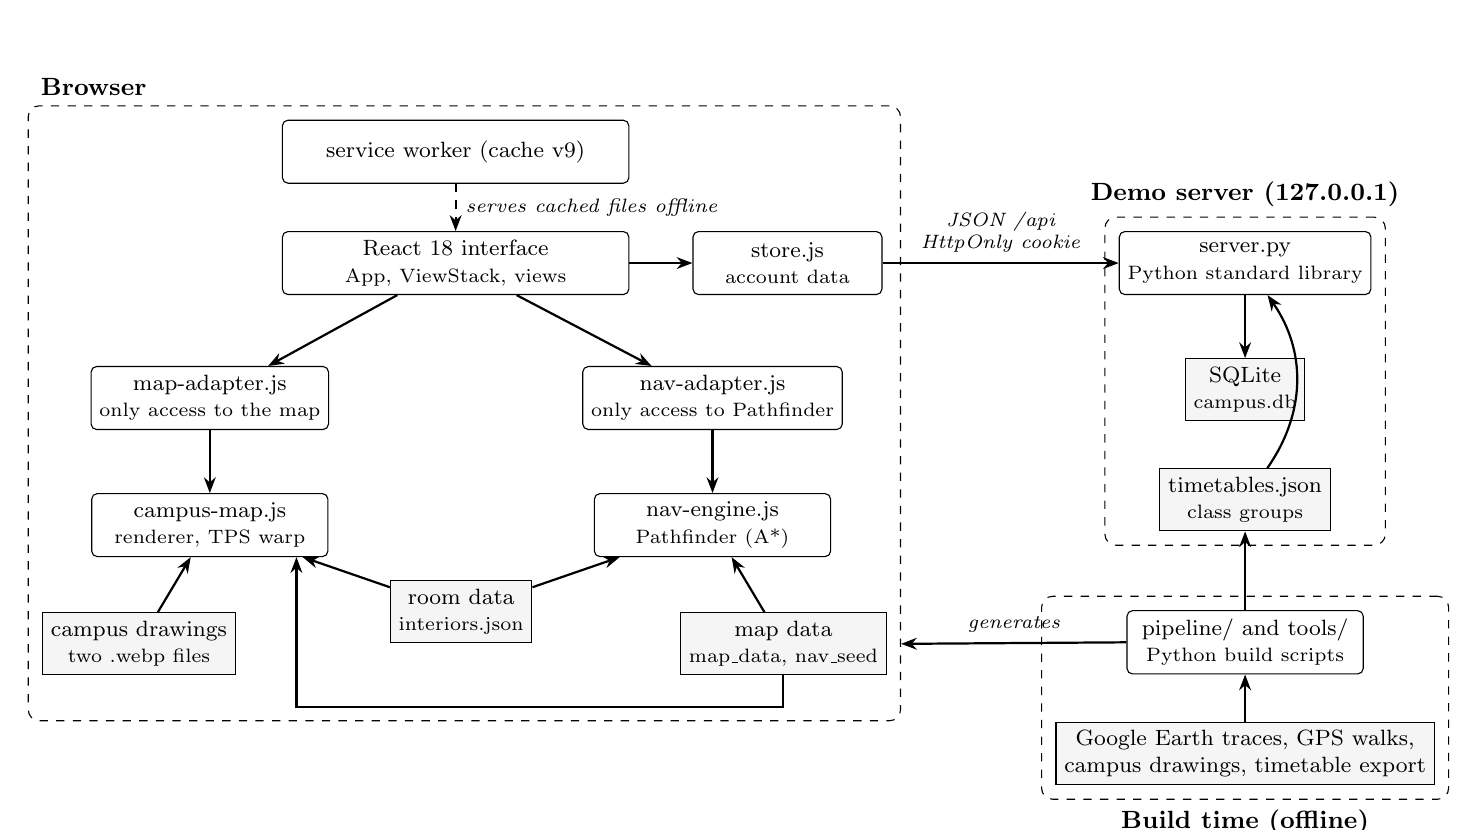
\begin{tikzpicture}[
  font=\footnotesize, node distance=4mm and 6mm,
  box/.style={draw, rounded corners=2pt, align=center, minimum height=8mm, inner sep=3pt, fill=white},
  data/.style={draw, align=center, minimum height=7mm, inner sep=3pt, fill=gray!8},
  zone/.style={draw, dashed, rounded corners=4pt, inner sep=5pt},
  arr/.style={-{Stealth[length=2mm]}, thick},
  lbl/.style={font=\scriptsize\itshape, align=center}]

  % ---- browser ----
  \node[box, minimum width=44mm] (ui) {React 18 interface\\\scriptsize App, ViewStack, views};
  \node[box, below left=9mm and -6mm of ui, minimum width=30mm] (ma) {map-adapter.js\\\scriptsize only access to the map};
  \node[box, below right=9mm and -6mm of ui, minimum width=30mm] (na) {nav-adapter.js\\\scriptsize only access to Pathfinder};
  \node[box, right=8mm of ui, minimum width=24mm] (st) {store.js\\\scriptsize account data};
  \node[box, below=8mm of ma, minimum width=30mm] (cm) {campus-map.js\\\scriptsize renderer, TPS warp};
  \node[box, below=8mm of na, minimum width=30mm] (ne) {nav-engine.js\\\scriptsize Pathfinder (A*)};
  \node[data, below=7mm of cm, xshift=-9mm] (dr) {campus drawings\\\scriptsize two .webp files};
  \node[data, below=7mm of $(cm)!0.5!(ne)$] (rd) {room data\\\scriptsize interiors.json};
  \node[data, below=7mm of ne, xshift=9mm] (md) {map data\\\scriptsize map\_data, nav\_seed};
  \node[box, above=6mm of ui, minimum width=44mm] (sw) {service worker (cache v9)};

  \draw[arr] (ui) -- (ma);
  \draw[arr] (ui) -- (na);
  \draw[arr] (ui) -- (st);
  \draw[arr] (ma) -- (cm);
  \draw[arr] (na) -- (ne);
  \draw[arr] (dr) -- (cm);
  \draw[arr] (rd) -- (cm);
  \draw[arr] (rd) -- (ne);
  \draw[arr] (md) -- (ne);
  % map data also feeds the renderer: routed below the data boxes
  \coordinate (low) at ($(md.south)+(0,-4mm)$);
  \draw[arr] (md.south) -- (low) -| ($(cm.south)+(11mm,0)$);
  \draw[arr, dashed] (sw) -- node[lbl, right] {serves cached files offline} (ui);

  \node[zone, fit=(sw)(ui)(ma)(na)(st)(cm)(ne)(dr)(rd)(md)(low), label={[font=\small\bfseries]above left:Browser}] (browser) {};

  % ---- server ----
  \node[box, right=30mm of st, minimum width=30mm] (srv) {server.py\\\scriptsize Python standard library};
  \node[data, below=8mm of srv] (db) {SQLite\\\scriptsize campus.db};
  \node[data, below=6mm of db] (tt) {timetables.json\\\scriptsize class groups};
  \draw[arr] (st) -- node[lbl, above, align=center] {JSON /api\\HttpOnly cookie} (srv);
  \draw[arr] (srv) -- (db);
  \draw[arr] (tt) to[bend right=35] (srv);
  \node[zone, fit=(srv)(db)(tt), label={[font=\small\bfseries]above:Demo server (127.0.0.1)}] {};

  % ---- build time ----
  \node[box, below=10mm of tt, minimum width=30mm] (pl) {pipeline/ and tools/\\\scriptsize Python build scripts};
  \node[data, below=6mm of pl, align=center] (src) {Google Earth traces, GPS walks,\\campus drawings, timetable export};
  \draw[arr] (src) -- (pl);
  \draw[arr] (pl.west) -- node[lbl, above] {generates} (md.east -| browser.east);
  \draw[arr] (pl) -- (tt);
  \node[zone, fit=(pl)(src), label={[font=\small\bfseries]below:Build time (offline)}] {};
\end{tikzpicture}
}
\caption{Architecture of BAC Maps, including Pathfinder, both adapters, the room data and the drawings}\label{fig:architecture}
\end{figure}

\begin{figure}[htbp]
\centering
\resizebox{0.95\textwidth}{!}{% Use case diagram. Solid: implemented. Dashed: planned, partial or descoped (see the legend).
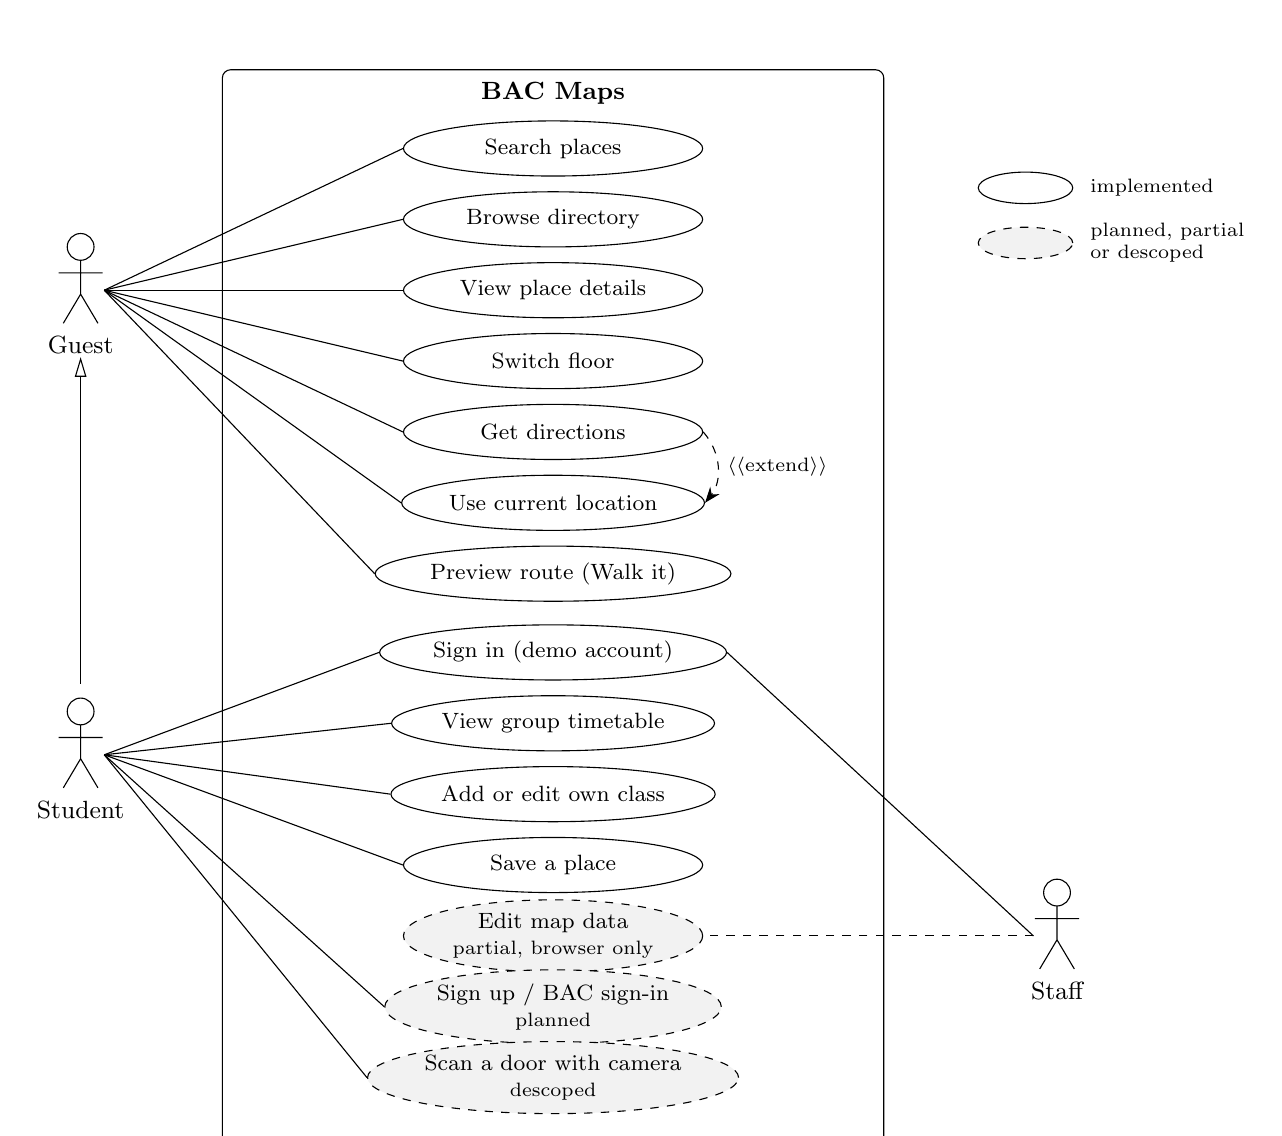
\begin{tikzpicture}[
  font=\footnotesize,
  uc/.style={draw, ellipse, align=center, minimum width=38mm, minimum height=7mm, inner sep=1pt, fill=white},
  ucp/.style={uc, dashed, fill=gray!10},
  actor/.style={align=center, font=\small},
  assoc/.style={thin},
  gen/.style={-{Triangle[open, length=2.5mm]}, thin}]

  \newcommand{\stick}[2]{% name, position
    \begin{scope}[shift={#2}]
      \draw (0,0.55) circle (0.17);
      \draw (0,0.38) -- (0,-0.05) (-0.28,0.22) -- (0.28,0.22) (0,-0.05) -- (-0.22,-0.42) (0,-0.05) -- (0.22,-0.42);
      \node[actor] at (0,-0.7) {#1};
    \end{scope}}

  % system boundary
  \draw[rounded corners=3pt] (-3.2,-9.6) rectangle (5.2,4.1);
  \node[font=\small\bfseries] at (1,3.8) {BAC Maps};

  % guest use cases
  \node[uc]  (u1) at (1,3.1)  {Search places};
  \node[uc]  (u2) at (1,2.2)  {Browse directory};
  \node[uc]  (u3) at (1,1.3)  {View place details};
  \node[uc]  (u4) at (1,0.4)  {Switch floor};
  \node[uc]  (u5) at (1,-0.5) {Get directions};
  \node[uc]  (u6) at (1,-1.4) {Use current location};
  \node[uc]  (u7) at (1,-2.3) {Preview route (Walk it)};
  % student use cases
  \node[uc]  (s1) at (1,-3.3) {Sign in (demo account)};
  \node[uc]  (s2) at (1,-4.2) {View group timetable};
  \node[uc]  (s3) at (1,-5.1) {Add or edit own class};
  \node[uc]  (s4) at (1,-6.0) {Save a place};
  % staff and planned
  \node[ucp] (p0) at (1,-6.9) {Edit map data\\\scriptsize partial, browser only};
  \node[ucp] (p1) at (1,-7.8) {Sign up / BAC sign-in\\\scriptsize planned};
  \node[ucp] (p2) at (1,-8.7) {Scan a door with camera\\\scriptsize descoped};

  \stick{Guest}{(-5,1.3)}
  \stick{Student}{(-5,-4.6)}
  \stick{Staff}{(7.4,-6.9)}

  \foreach \u in {u1,u2,u3,u4,u5,u6,u7} \draw[assoc] (-4.7,1.3) -- (\u.west);
  \foreach \u in {s1,s2,s3,s4,p1,p2} \draw[assoc] (-4.7,-4.6) -- (\u.west);
  \draw[gen] (-5,-3.7) -- (-5,0.45);
  \draw[assoc, dashed] (7.1,-6.9) -- (p0.east);
  \draw[assoc] (7.1,-6.9) -- (s1.east);

  \draw[dashed, -{Stealth[length=2mm]}] (u5.east) to[bend left=40] node[right, font=\scriptsize] {$\langle\langle$extend$\rangle\rangle$} (u6.east);

  % legend
  \node[uc, minimum width=12mm, minimum height=4mm] at (7.0,2.6) {};
  \node[right, font=\scriptsize] at (7.7,2.6) {implemented};
  \node[ucp, minimum width=12mm, minimum height=4mm] at (7.0,1.9) {};
  \node[right, font=\scriptsize, align=left] at (7.7,1.9) {planned, partial\\or descoped};
\end{tikzpicture}
}
\caption{Use case diagram. Dashed use cases are planned, partial or descoped}\label{fig:usecase}
\end{figure}

\begin{figure}[htbp]
\centering
\resizebox{0.8\textwidth}{!}{% Activity diagram: getting directions to a place
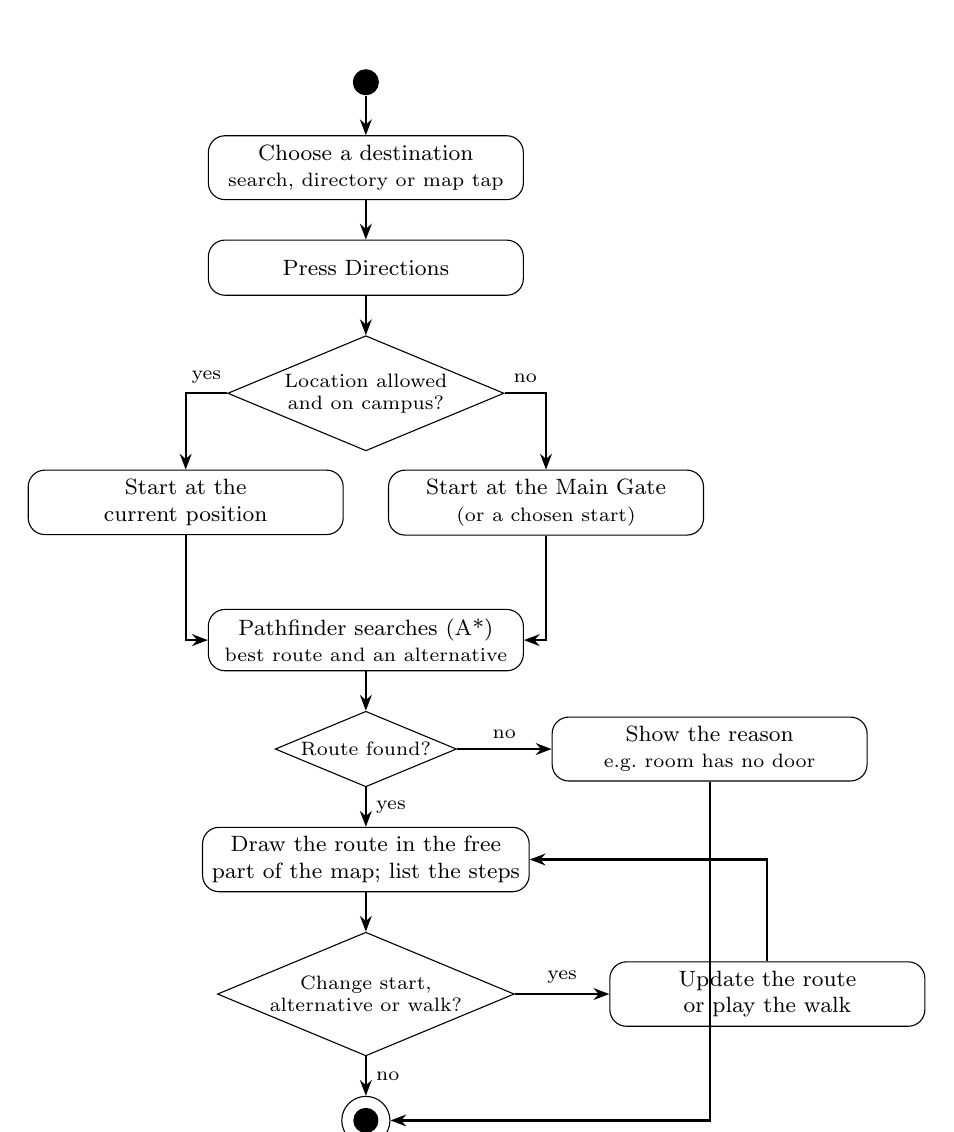
\begin{tikzpicture}[
  font=\footnotesize, node distance=5mm and 8mm,
  act/.style={draw, rounded corners=6pt, align=center, minimum width=40mm, minimum height=7mm, fill=white},
  dec/.style={draw, diamond, aspect=2.4, align=center, inner sep=1pt, font=\scriptsize},
  arr/.style={-{Stealth[length=2mm]}, thick},
  lbl/.style={font=\scriptsize}]

  \node[circle, fill=black, minimum size=3mm] (start) {};
  \node[act, below=of start] (a1) {Choose a destination\\\scriptsize search, directory or map tap};
  \node[act, below=of a1] (a2) {Press Directions};
  \node[dec, below=of a2] (d1) {Location allowed\\and on campus?};
  \node[act, below left=6mm and -6mm of d1] (a3) {Start at the\\current position};
  \node[act, below right=6mm and -6mm of d1] (a4) {Start at the Main Gate\\\scriptsize (or a chosen start)};
  \node[act, below=20mm of d1] (a5) {Pathfinder searches (A*)\\\scriptsize best route and an alternative};
  \node[dec, below=of a5] (d2) {Route found?};
  \node[act, right=12mm of d2] (a6) {Show the reason\\\scriptsize e.g.\ room has no door};
  \node[act, below=of d2] (a7) {Draw the route in the free\\part of the map; list the steps};
  \node[dec, below=of a7] (d3) {Change start,\\alternative or walk?};
  \node[act, right=12mm of d3] (a8) {Update the route\\or play the walk};
  \node[circle, draw, inner sep=1.6pt, below=of d3] (end) {\tikz\fill (0,0) circle (1.6mm);};

  \draw[arr] (start) -- (a1);
  \draw[arr] (a1) -- (a2);
  \draw[arr] (a2) -- (d1);
  \draw[arr] (d1) -| node[lbl, above, pos=0.25] {yes} (a3);
  \draw[arr] (d1) -| node[lbl, above, pos=0.25] {no} (a4);
  \draw[arr] (a3) |- (a5);
  \draw[arr] (a4) |- (a5);
  \draw[arr] (a5) -- (d2);
  \draw[arr] (d2) -- node[lbl, above] {no} (a6);
  \draw[arr] (d2) -- node[lbl, right] {yes} (a7);
  \draw[arr] (a7) -- (d3);
  \draw[arr] (d3) -- node[lbl, above] {yes} (a8);
  \draw[arr] (a8.north) |- (a7.east);
  \draw[arr] (d3) -- node[lbl, right] {no} (end);
  \draw[arr] (a6.south) |- (end.east);
\end{tikzpicture}
}
\caption{Activity diagram for getting directions}\label{fig:activity}
\end{figure}

\begin{figure}[htbp]
\centering
\resizebox{0.85\textwidth}{!}{% Entity-relationship diagram of the demo database (server/db.py)
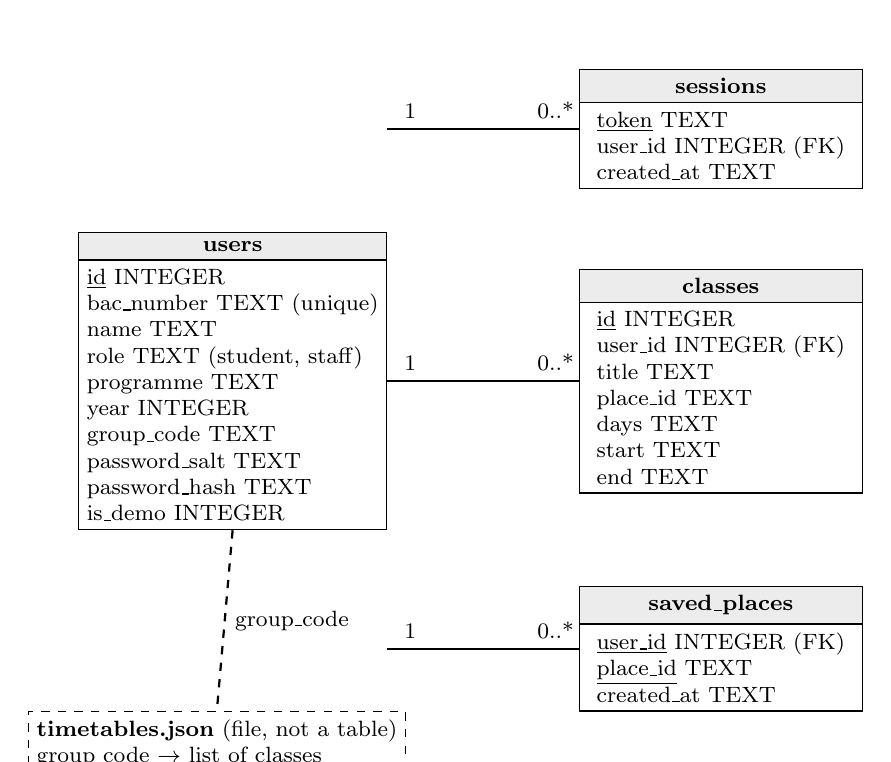
\begin{tikzpicture}[
  font=\footnotesize,
  ent/.style={draw, rectangle split, rectangle split parts=2, align=left, inner sep=3pt, minimum width=36mm,
              rectangle split part fill={gray!15, white}},
  rel/.style={thick}]

  \node[ent] (users) at (0,0) {\textbf{users}
    \nodepart{two}\underline{id} INTEGER\\ bac\_number TEXT (unique)\\ name TEXT\\ role TEXT (student, staff)\\ programme TEXT\\ year INTEGER\\ group\_code TEXT\\ password\_salt TEXT\\ password\_hash TEXT\\ is\_demo INTEGER};
  \node[ent] (sessions) at (6.2,3.2) {\textbf{sessions}
    \nodepart{two}\underline{token} TEXT\\ user\_id INTEGER (FK)\\ created\_at TEXT};
  \node[ent] (classes) at (6.2,0) {\textbf{classes}
    \nodepart{two}\underline{id} INTEGER\\ user\_id INTEGER (FK)\\ title TEXT\\ place\_id TEXT\\ days TEXT\\ start TEXT\\ end TEXT};
  \node[ent] (saved) at (6.2,-3.4) {\textbf{saved\_places}
    \nodepart{two}\underline{user\_id} INTEGER (FK)\\ \underline{place\_id} TEXT\\ created\_at TEXT};
  \node[draw, dashed, align=left, inner sep=3pt] (tt) at (-0.2,-4.6) {\textbf{timetables.json} (file, not a table)\\ group code $\rightarrow$ list of classes};

  \draw[rel] (users.east |- sessions) -- node[above, pos=0.12] {1} node[above, pos=0.88] {0..*} (sessions.west);
  \draw[rel] (users.east |- classes) -- node[above, pos=0.12] {1} node[above, pos=0.88] {0..*} (classes.west);
  \draw[rel] (users.east |- saved) -- node[above, pos=0.12] {1} node[above, pos=0.88] {0..*} (saved.west);
  \draw[dashed, thick] (users.south) -- node[right] {group\_code} (tt.north);
\end{tikzpicture}
}
\caption{Entity-relationship diagram of the demonstration database}\label{fig:er}
\end{figure}

\subsection{Timeline and team contributions}
\placeholder{project timeline: the main phases and their dates (Table~\ref{tab:timeline})}

\begin{table}[htbp]
\centering\tablespacing
\caption{Timeline and team contributions}\label{tab:timeline}
\begin{tabular}{p{4.5cm}p{9.5cm}}
\toprule
Team member & Main contributions \\
\midrule
Kaelo Kealeboga Selome & \placeholder{contributions} \\
Monyana Bianca Kedukaetswe & \placeholder{contributions} \\
Larona Mothame & \placeholder{contributions} \\
Katlo Tutwane & \placeholder{contributions} \\
Abigail Mototegi & \placeholder{contributions} \\
\bottomrule
\end{tabular}
\end{table}

\subsection{Data collection methods and description of data sources}
\begin{itemize}
  \item \textbf{Google Earth traces:} 22 buildings, 18 paths, 10 areas and 3 roads traced over satellite imagery and exported as KML.
  \item \textbf{Measured walks:} ten walks recorded on site with GPS (for example \emph{Main Gate to the student entrance}), marked as verified paths.
  \item \textbf{Campus drawings:} an illustrated campus drawing and a ground-floor drawing of the Main Building, both marked as concepts not to scale, used for what is where (room names, order, stairs).
  \item \textbf{Timetable export:} the SCIS 2026--2027 Semester 1 timetable exported from primetimetable.com, giving five class groups and 40 weekly classes.
\end{itemize}

\subsection{Rationale for using secondary data}
Surveying the campus or modelling the buildings was not possible within the project's time and budget. Satellite imagery, the college's drawings and its published timetable already existed, cover the whole campus and can be updated when the college changes. The measured walks were collected to check the secondary data where it matters most, on the main approaches from the gate.

\subsection{Data selection criteria}
A feature was included when it could be seen on the imagery or a drawing and named by the team. Room names were taken from the drawings; a room's shape was taken from the traced building footprint, because the drawings are not to scale. A staircase was connected only when both drawings agree: the stairs between the CAF and the lecture theatre appear on only one drawing and are therefore left out until confirmed. Only timetable rooms that match a mapped place are linked (five room codes).

\subsection{Data analysis procedures}
Python build scripts turn the KML traces and walks into \texttt{map\_data.json}, build the rooms, doors and stairs into \texttt{interiors.json}, and convert the timetable export into \texttt{timetables.json}. Rooms are made by dividing the Main Building's footprint, minus a 2.8\,m corridor (measured on site), between the rooms named on the drawings. The drawings are placed on the map with a thin-plate spline \citep{bookstein1989} fitted to 82 control points:
\begin{equation}\label{eq:tps}
  \mathbf{p}(\mathbf{x}) = \mathbf{A}\mathbf{x} + \mathbf{b} + \sum_{i=1}^{n} \mathbf{w}_i\, r_i^{2} \ln r_i, \qquad r_i = \lVert \mathbf{x} - \mathbf{c}_i \rVert
\end{equation}
where $\mathbf{x}$ is a ground position in metres, $\mathbf{p}(\mathbf{x})$ the matching pixel on the drawing, $\mathbf{A}$ and $\mathbf{b}$ an affine transform, $\mathbf{c}_i$ the $n=82$ control points and $\mathbf{w}_i$ their fitted weights. Equation~\ref{eq:tps} only places the existing drawings and routes onto each other; it does not draw the map.

\subsection{Evaluation of data quality}\label{sec:quality}
The fitted drawing lies a median of 1.6\,m and at most 13.2\,m from its control points. The campus drawing matches 17 traced building labels with a median error of 1.5\,m (worst 6.7\,m). All 40 rooms are marked approximate: the drawings place the south-east wing 4--8\,m east of the satellite footprint, and rooms there were fitted to the footprint. Storey counts for buildings other than the Main Building are assumed to be one, and two stair positions are estimated from an evacuation sign. Office~3 has no corridor wall in the footprint, so it has no door.

\section{Requirements Catalogue and Feature Selection}\label{sec:catalogue}
The original catalogue (FR-01 to FR-13, NFR-01 to NFR-09) was built around a camera that would recognise a room's door and check it against the timetable. That system was not implemented. The catalogue was therefore revised to the 20 functional requirements in Table~\ref{tab:fr}, prioritised with MoSCoW (Must, Should, Could, Won't). Each revised requirement keeps a link to the original identifier it replaces. The descoped requirements are listed in Table~\ref{tab:descoped}, and the non-functional requirements in Table~\ref{tab:nfr}. Appendix~\ref{app:cards} gives the full cards with acceptance criteria.

{\tablespacing
\begin{longtable}{p{1.3cm}p{8.6cm}p{1.4cm}p{2.2cm}}
\caption{Revised functional requirements}\label{tab:fr}\\
\toprule
ID & The system shall \ldots & Priority & Original \\
\midrule\endfirsthead
\toprule
ID & The system shall \ldots & Priority & Original \\
\midrule\endhead
\bottomrule\endfoot
FR-01 & display an interactive map of the campus that can be panned, zoomed and reset & Must & FR-01 \\
FR-02 & switch between All, Ground and First floor without reloading & Must & FR-02 \\
FR-03 & search buildings, rooms and facilities by name & Must & new \\
FR-04 & offer quick category picks and a directory grouped by category & Should & new \\
FR-05 & select a building or room by tapping it on the map & Should & new \\
FR-06 & show a place card with category, building and floor, and actions for directions, saving and showing on the map & Should & FR-06 (revised) \\
FR-07 & compute a walking route from an entrance gate to a chosen room & Must & FR-05 \\
FR-08 & route across floors through mapped doors and stairs, with steps grouped by floor & Must & FR-05 \\
FR-09 & offer an alternative route when a distinct one exists & Could & new \\
FR-10 & let the user change the start and destination of a route & Should & new \\
FR-11 & start from the user's position when on campus, otherwise from the Main Gate & Could & new \\
FR-12 & preview a route with an animated walk and pin a selected step on the map & Could & new \\
FR-13 & explain why no route exists when a place cannot be reached & Must & new \\
FR-14 & keep the shown route clear of the directions panel & Should & new (C3) \\
FR-15 & let a student sign in and out so data is tied to one account & Must & FR-12 \\
FR-16 & show a signed-in student's class-group timetable by day & Must & FR-03 (revised) \\
FR-17 & let a student add, edit and delete their own classes & Should & FR-03 \\
FR-18 & show the student's next class with directions to its room & Must & FR-04 (revised) \\
FR-19 & let a student save places and list them in the profile & Should & new \\
FR-20 & let staff correct map data (doors, links) without changing code & Could & FR-11 (revised) \\
\end{longtable}}

\subsection{Descoped requirements}\label{sec:descoped}
The camera requirements FR-07, FR-08 and FR-09 were rated Must in the original catalogue. They were descoped because the prerequisites do not exist in the project: there is no database of door photographs for the 40 rooms, no vision service has been chosen or tested, and sending camera images of the campus to an outside service would need the college's permission. Delivering the map and routes, on which the camera feature would also depend, was given priority. \placeholder{the team's own recorded reason and date for descoping the camera, if different}

\begin{table}[htbp]
\centering\tablespacing
\caption{Requirements from the original catalogue that were descoped or not implemented}\label{tab:descoped}
\begin{tabular}{p{1.6cm}p{7.2cm}p{1.4cm}p{3.6cm}}
\toprule
Original & Requirement & Priority & Status and reason \\
\midrule
FR-07 & Capture a live frame of a door with the camera & Must & Descoped (see above) \\
FR-08 & Match a door image against room photos with a vision API ($\geq$90\% correct) & Must & Descoped; no photo set \\
FR-09 & Cross-check a recognised room against the timetable & Must & Descoped; depends on FR-08 \\
NFR-02 & Camera result within 3 seconds & -- & Descoped with FR-07 to FR-09 \\
FR-10 & Arrival alert before the next class & Should & Not implemented \\
FR-13 & Show room capacity when vacant & Could & Not implemented; no capacity data \\
\bottomrule
\end{tabular}
\end{table}

\begin{table}[htbp]
\centering\tablespacing
\caption{Non-functional requirements (revised)}\label{tab:nfr}
\begin{tabular}{p{1.5cm}p{12.5cm}}
\toprule
ID & Requirement \\
\midrule
NFR-01 & The map shall display, a floor change shall take effect and a route shall appear within 2 seconds. \\
NFR-03 & The application shall be usable on Android and iOS phones and on desktop browsers. \\
NFR-04 & Account data shall be stored securely and be readable and changeable only by its owner. \\
NFR-05 & The system shall remain available during peak class-changeover periods. \\
NFR-06 & Rooms and paths shall be updatable through the build pipeline without code changes. \\
NFR-07 & The interface shall follow accessible design practice: contrast, text size and controls at least 44\,px tall. \\
NFR-08 & The system shall use React~18 with Vite for the interface, JavaScript for the map and route engine, Python for the build scripts and demonstration server, and SQLite for account data. \\
NFR-09 & The prototype shall be delivered within the 16-week project timeline. \\
NFR-10 & After one visit, the map and routes shall work without a network connection (new). \\
\bottomrule
\end{tabular}
\end{table}

\section{Data Analysis Techniques}
\begin{itemize}
  \item \textbf{Automated suites:} five Node.js suites test Pathfinder (navigation, interiors, scenarios, walks, concurrency) and three Playwright suites test the application in Microsoft Edge (site, profile, floors). The site and profile suites start the demonstration server with a temporary database.
  \item \textbf{Wall sampling:} every route is sampled every 25\,cm and each sample is checked to lie on walkable ground and outside rooms except through doors.
  \item \textbf{Visibility measurement:} the share of the route's on-screen length that is not covered by the panel, measured on desktop and phone sizes.
  \item \textbf{Timings:} measured inside the page with \texttt{performance.now()}, five runs per case, cache disabled, on a local server and with a simulated 4G-like connection (9\,Mbit/s down, 1.5\,Mbit/s up, 60\,ms latency) and a 4$\times$ processor slowdown.
  \item \textbf{Security checks:} direct API calls with wrong passwords, a second account, invalid input and requests for private files.
  \item \textbf{Manual checks:} features without an automated check (marked \emph{manual} in Table~\ref{tab:cases}) were exercised by hand in Edge and recorded in the screenshot tour.
\end{itemize}

\section{Ethical Considerations}
Only dummy demonstration accounts exist; no student's real data is stored. Passwords are stored as salted PBKDF2-SHA256 hashes with 200\,000 rounds, and the session is an HttpOnly, SameSite=Strict cookie that expires after seven days. The user's position is requested through the browser's permission prompt, used only in the browser to choose the start of a route, and never sent to the server. The timetable lists lecturers by initials only. \placeholder{whether the college gave permission to use its campus drawings and timetable export}

% =====================================================================
\chapter{Results and Analysis}\label{ch:results}

\section{Presentation of Key Findings}

\subsection{The application}
Figure~\ref{fig:overview} gives an overview of the application's main screens. On desktop, a search bar and a panel sit over the map; on a phone, the panel becomes a card at the bottom of the screen. Figures~\ref{fig:search} to~\ref{fig:phone} show the features in the revised catalogue.

\begin{figure}[htbp]
\centering
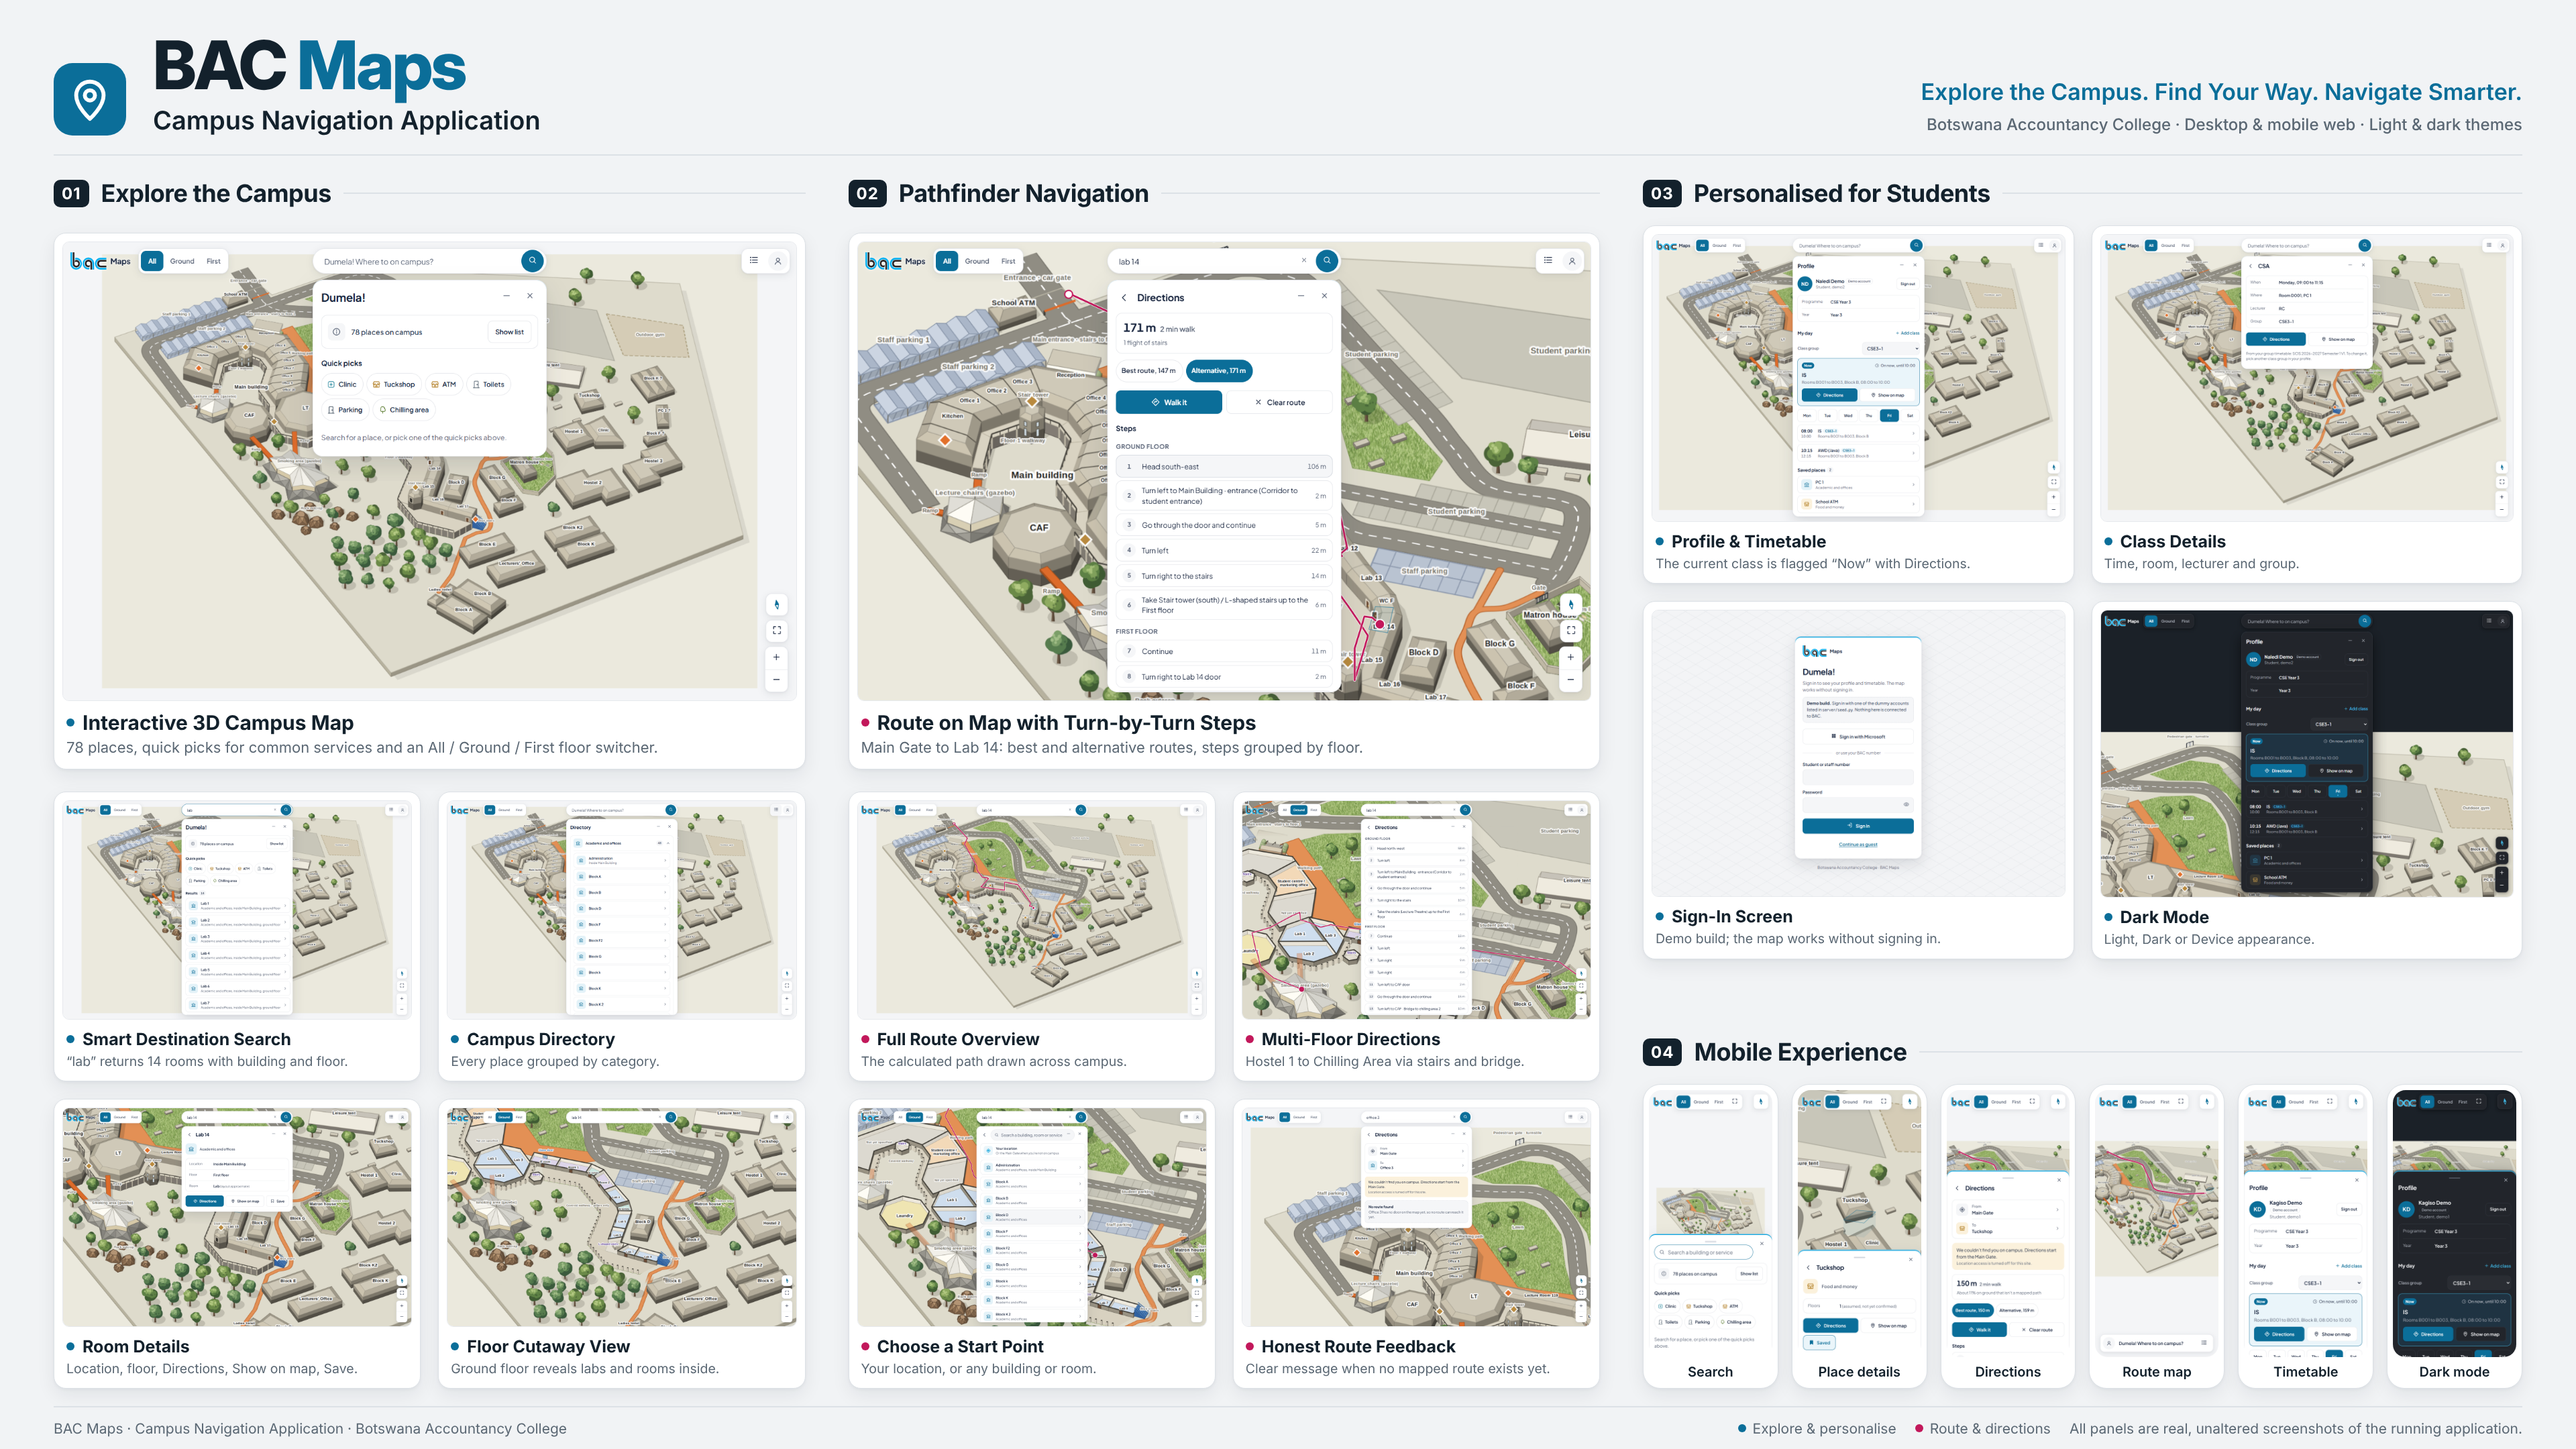
\includegraphics[width=\textwidth]{figures/bac-maps-collage.png}
\caption{Overview of the main screens of BAC Maps}\label{fig:overview}
\end{figure}

\begin{figure}[htbp]
\centering
\begin{subfigure}{0.49\textwidth}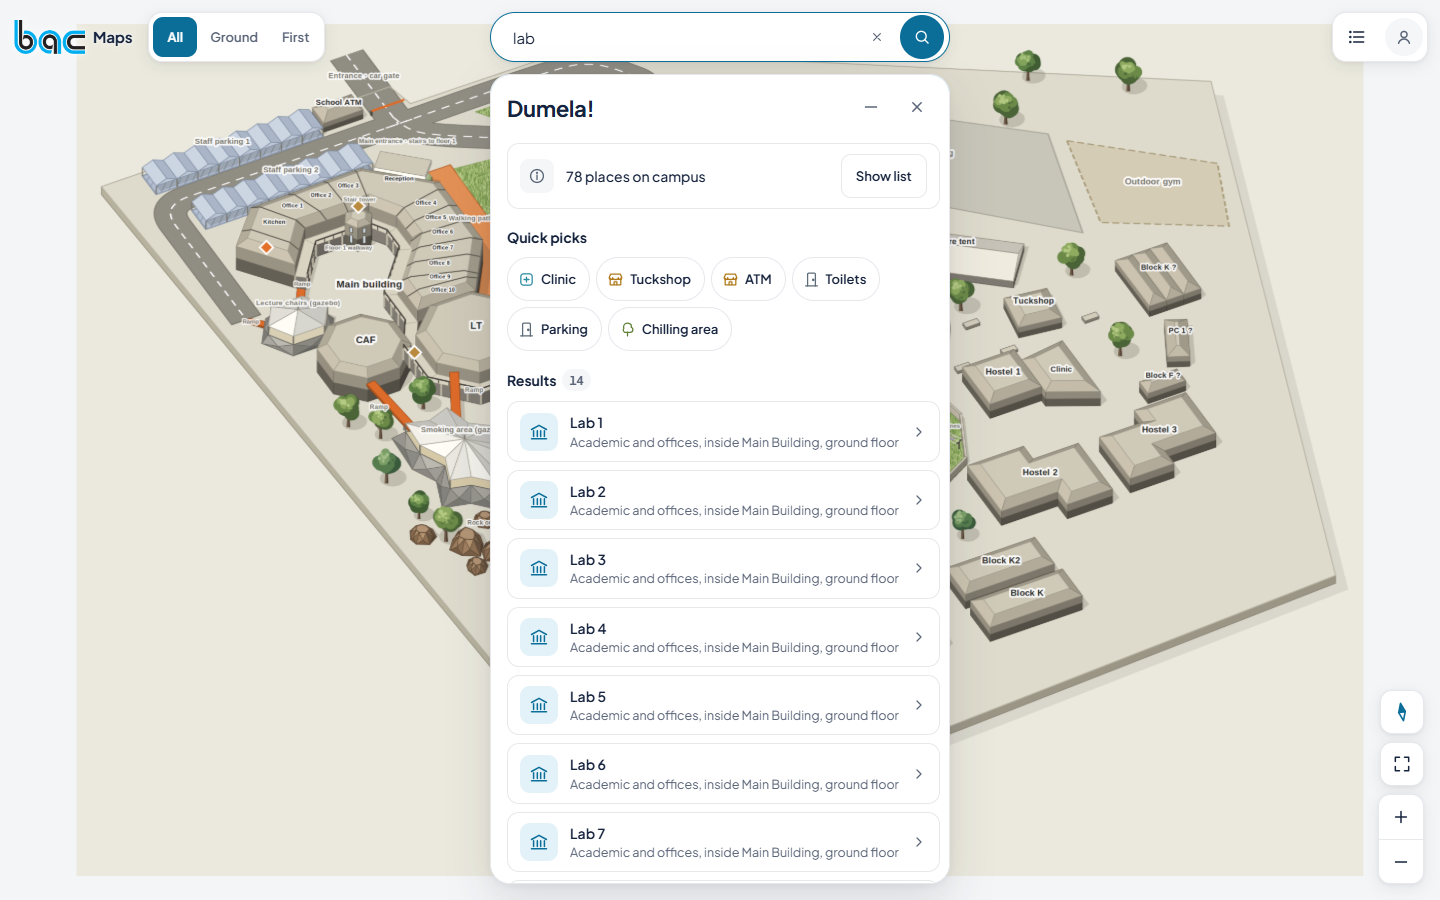
\includegraphics[width=\linewidth]{figures/tour/02-search-results-rooms-and-labs.png}\caption{Search results for ``lab'' (FR-03)}\end{subfigure}\hfill
\begin{subfigure}{0.49\textwidth}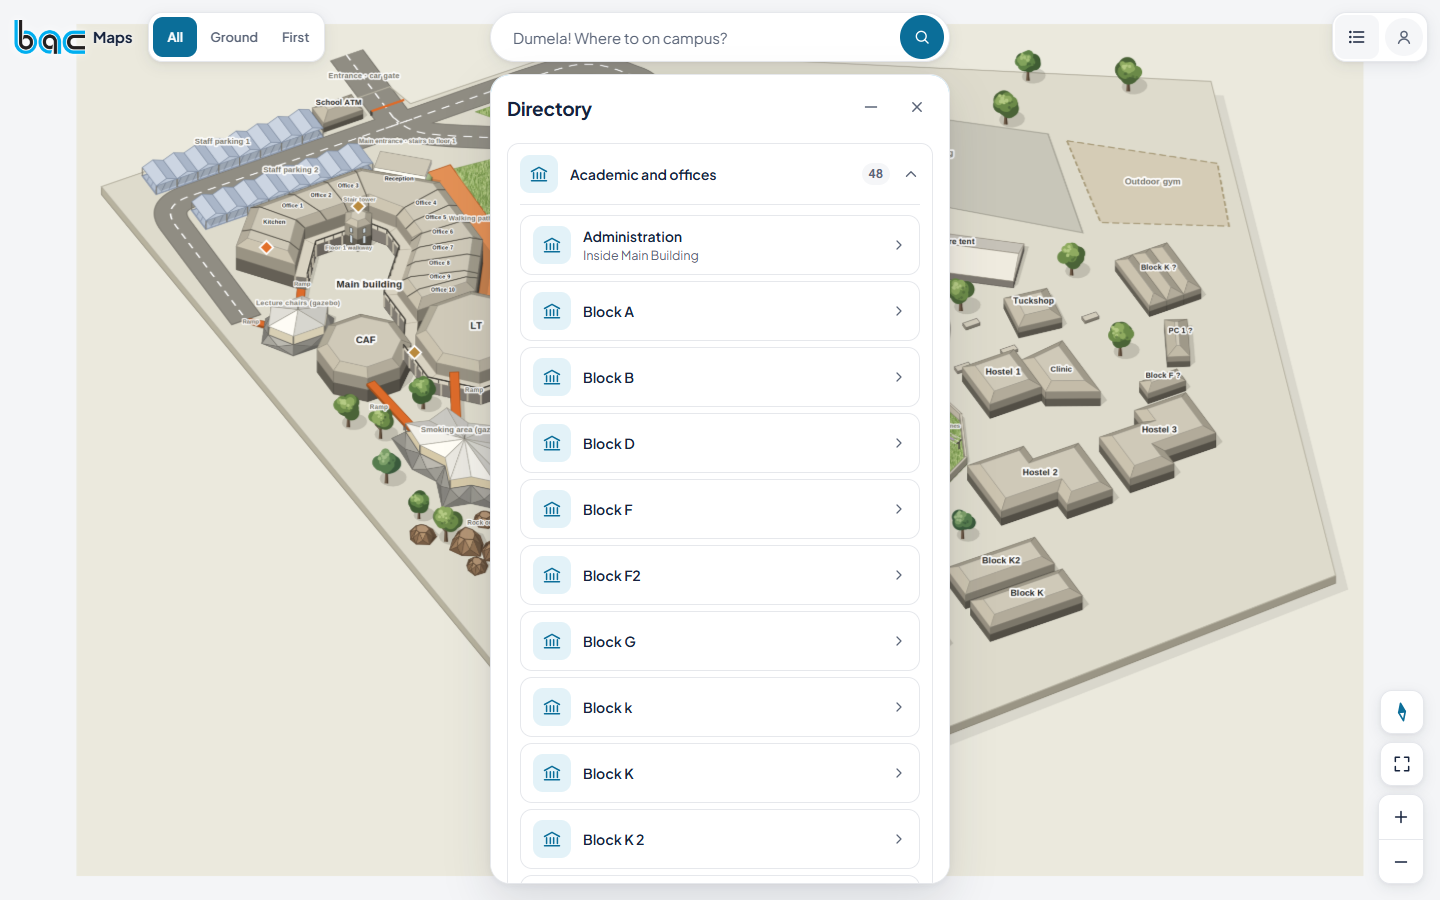
\includegraphics[width=\linewidth]{figures/tour/04-directory-by-category.png}\caption{Directory by category (FR-04)}\end{subfigure}\\[2mm]
\begin{subfigure}{0.49\textwidth}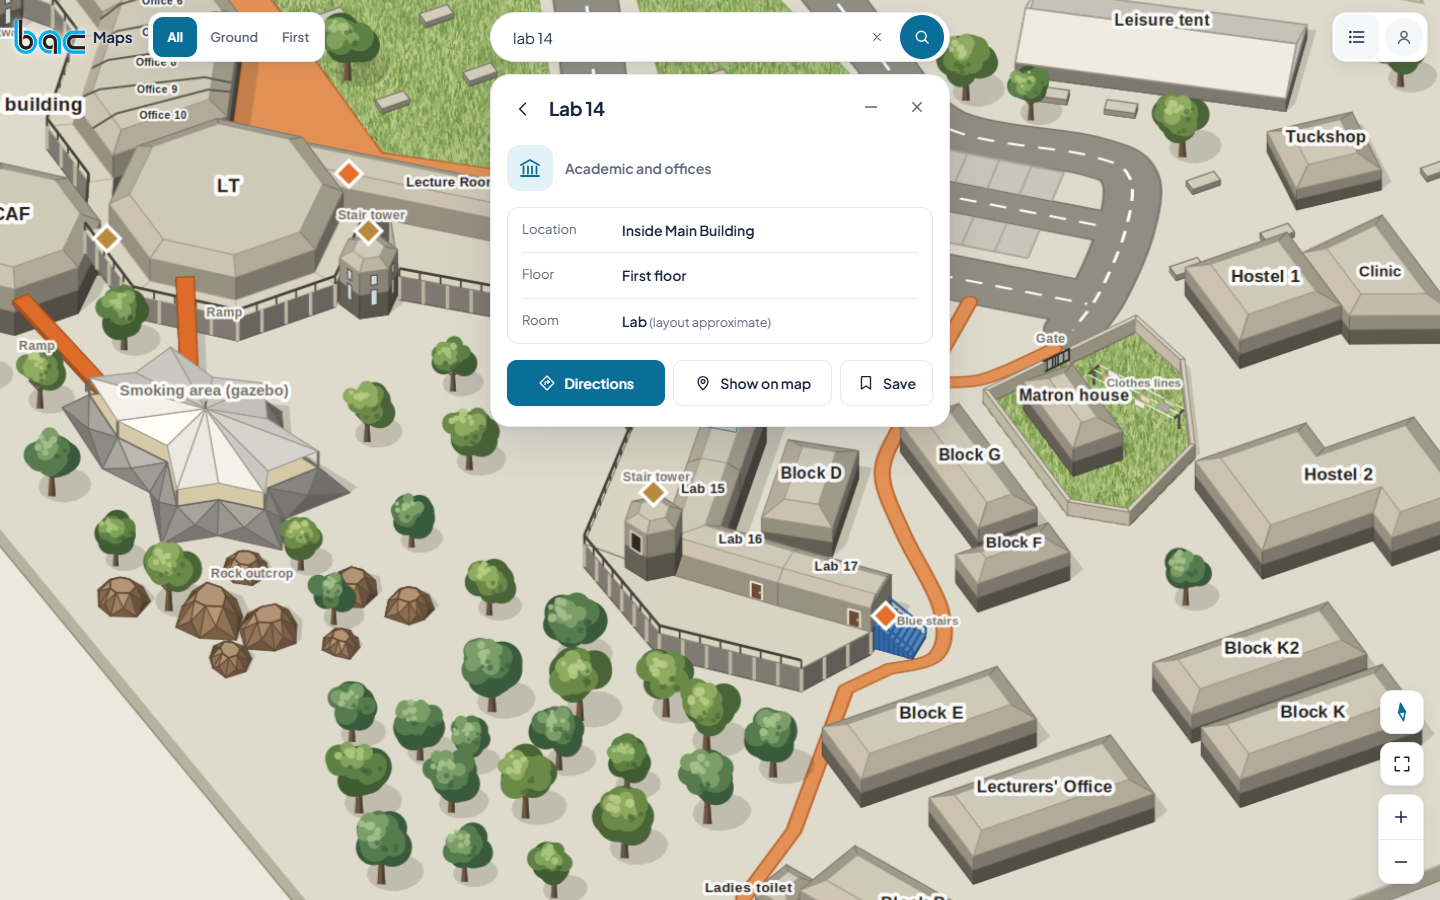
\includegraphics[width=\linewidth]{figures/tour/06-room-details-first-floor.png}\caption{Room card for Lab 14 (FR-06)}\end{subfigure}\hfill
\begin{subfigure}{0.49\textwidth}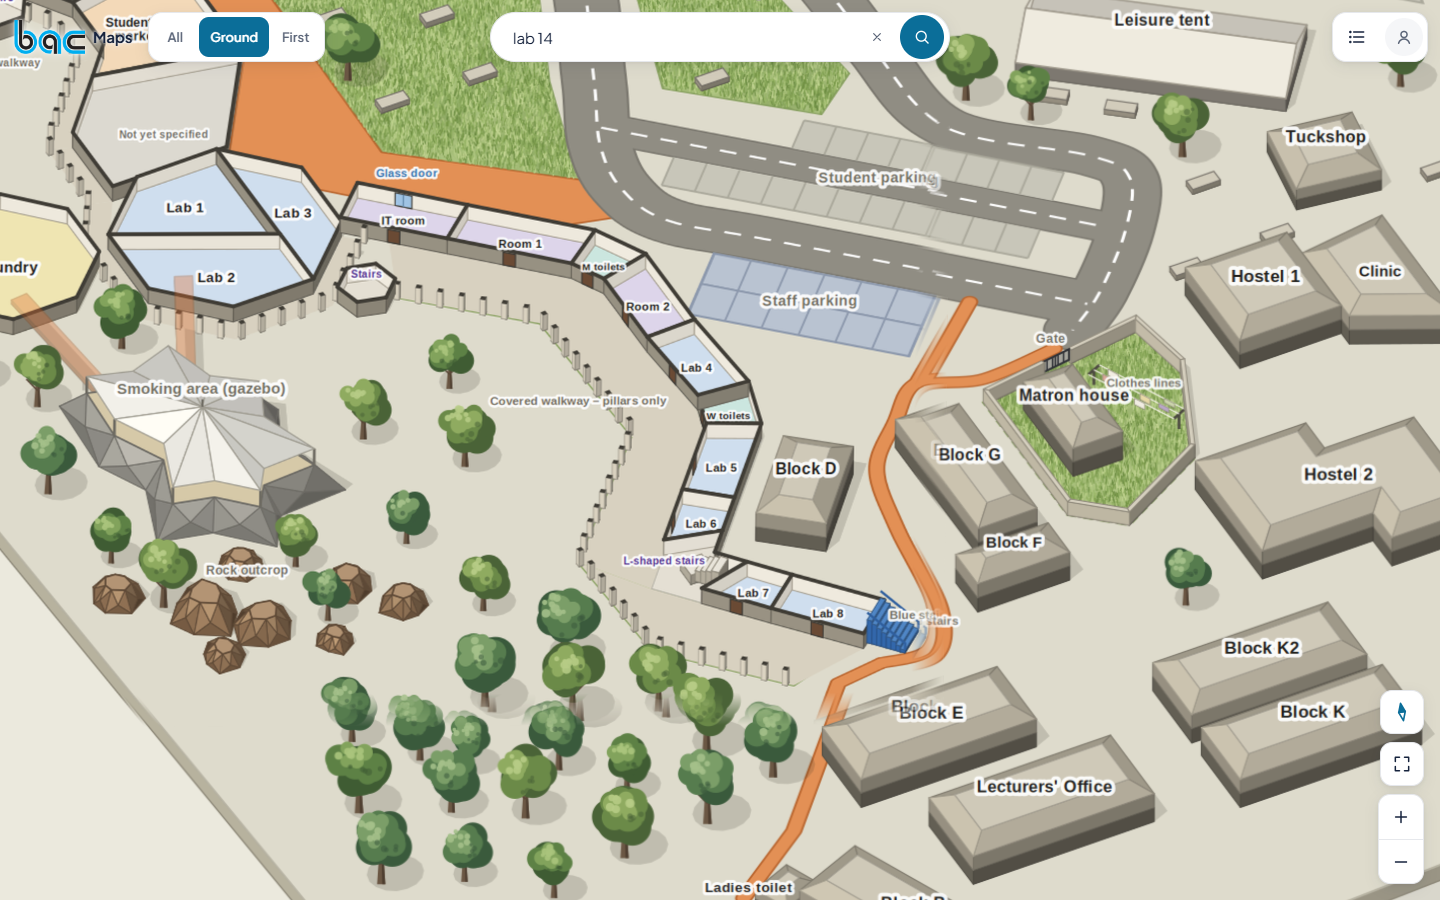
\includegraphics[width=\linewidth]{figures/tour/07-floor-ground-cutaway.png}\caption{Ground floor shown (FR-02)}\end{subfigure}
\caption{Finding a place: search, directory, place card and floors}\label{fig:search}
\end{figure}

\begin{figure}[htbp]
\centering
\begin{subfigure}{0.49\textwidth}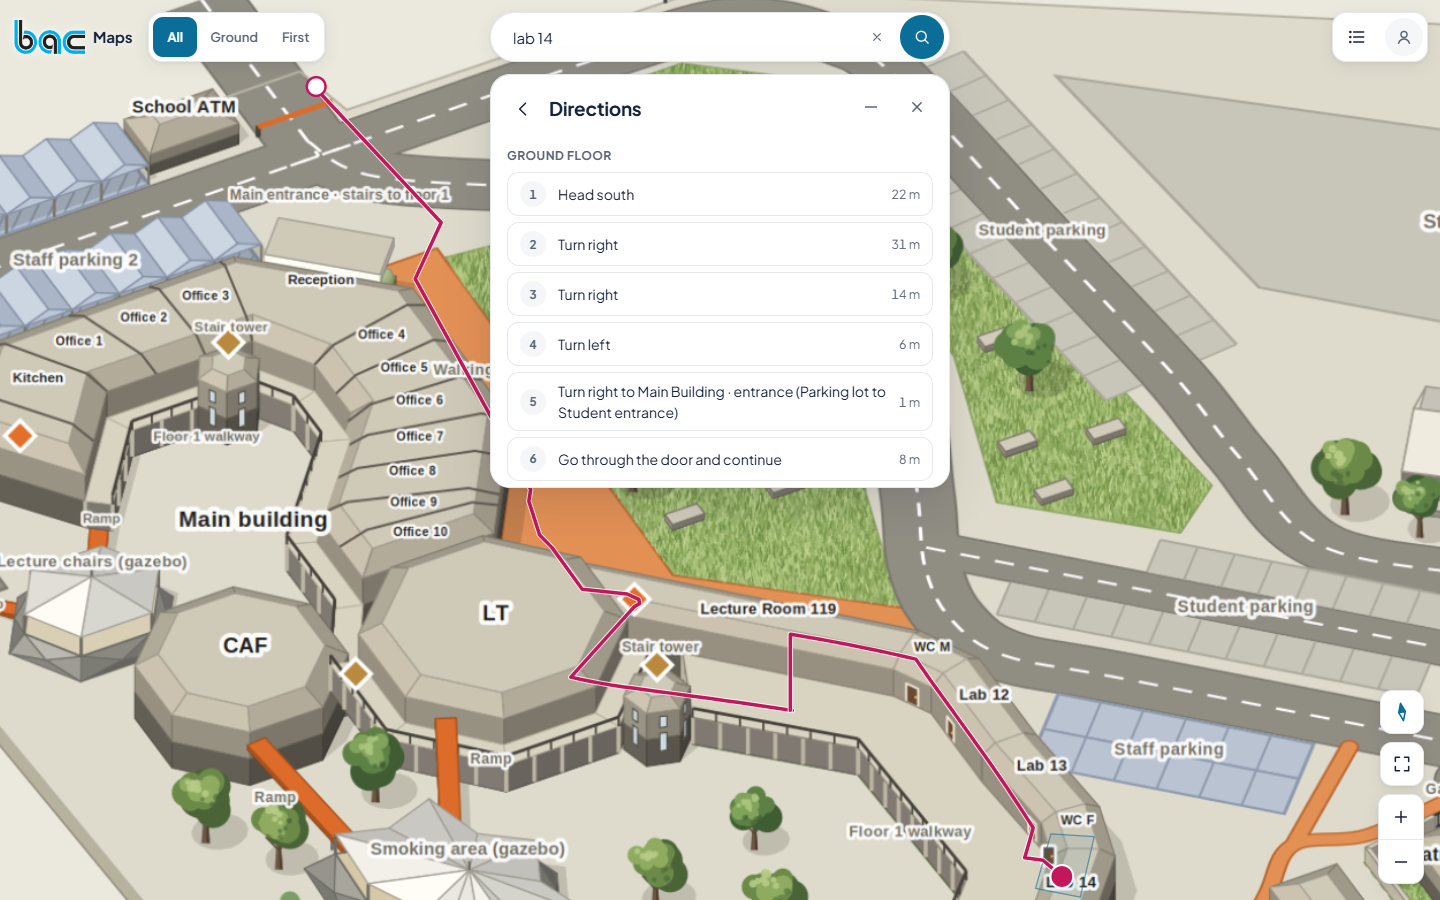
\includegraphics[width=\linewidth]{figures/tour/12-directions-steps-by-floor.png}\caption{Steps grouped by floor (FR-08)}\end{subfigure}\hfill
\begin{subfigure}{0.49\textwidth}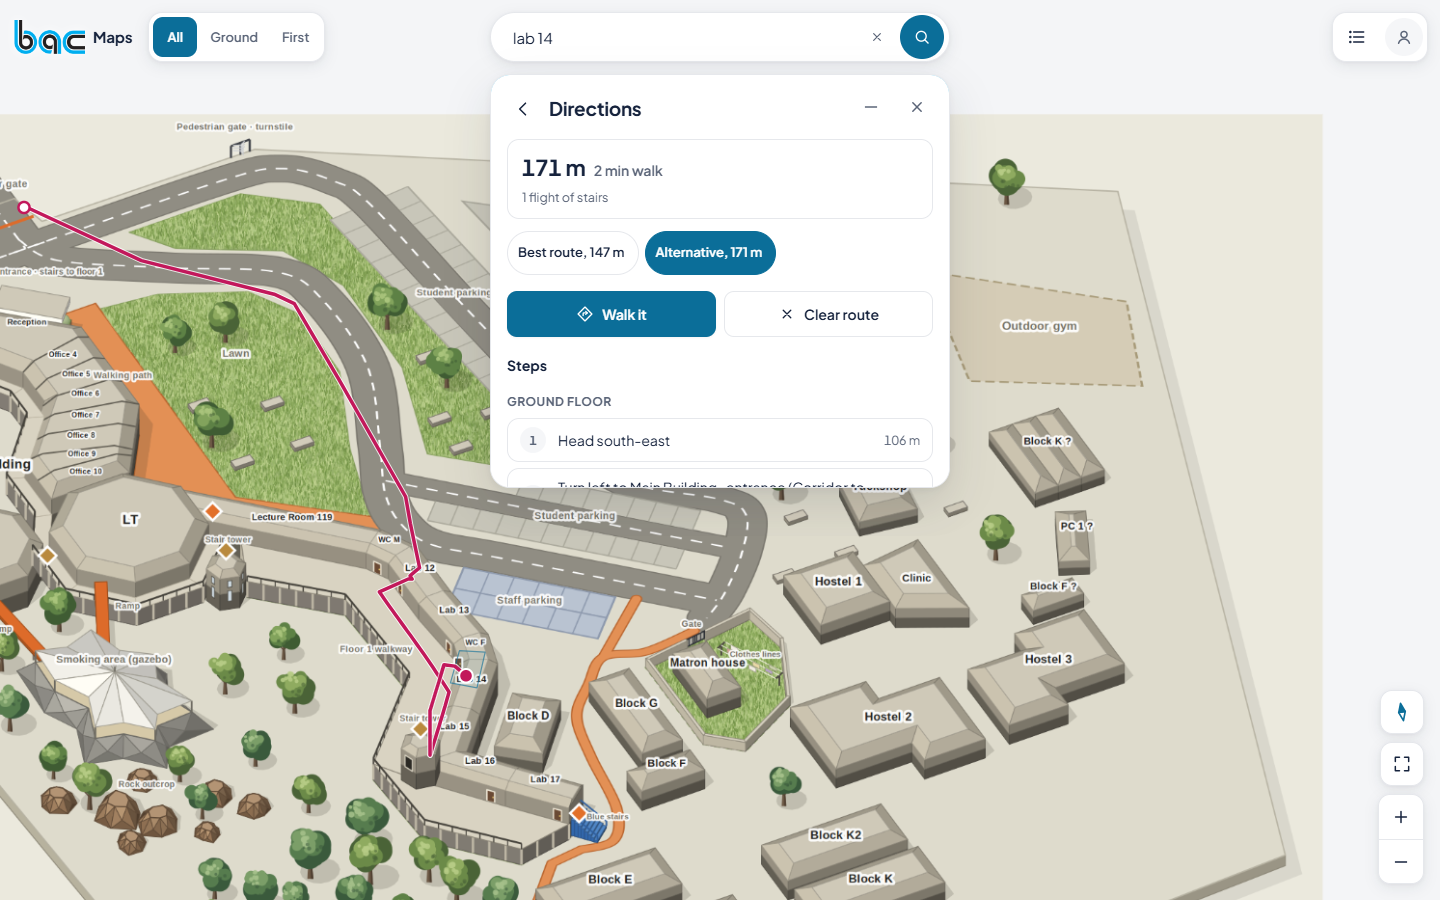
\includegraphics[width=\linewidth]{figures/tour/13-directions-alternative-route.png}\caption{Alternative route (FR-09)}\end{subfigure}\\[2mm]
\begin{subfigure}{0.49\textwidth}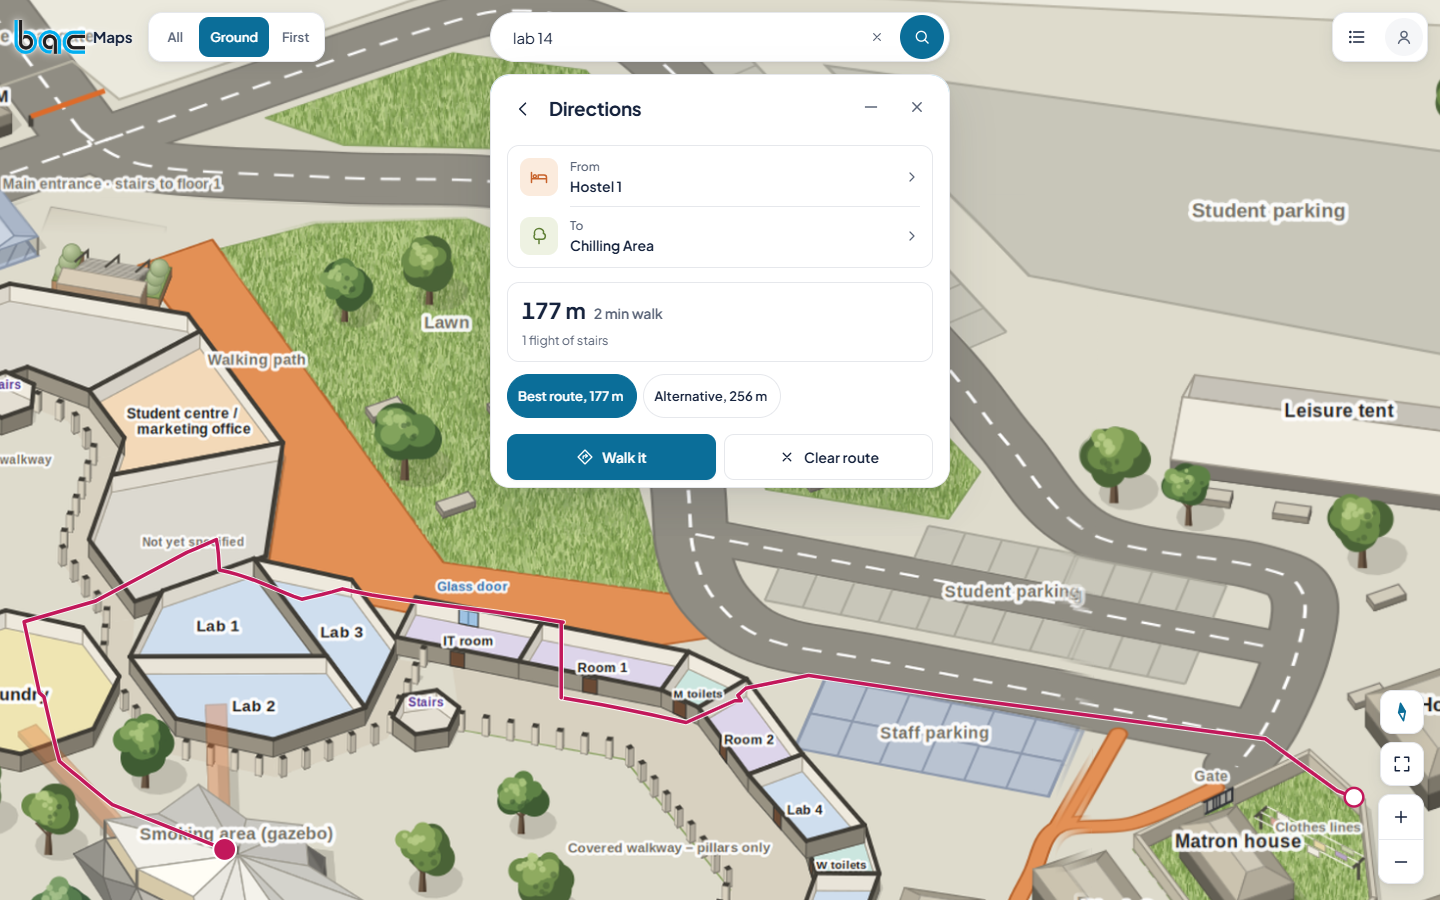
\includegraphics[width=\linewidth]{figures/tour/17-route-hostel-1-to-chilling-area-via-bridge.png}\caption{Changed start and end (FR-10)}\end{subfigure}\hfill
\begin{subfigure}{0.49\textwidth}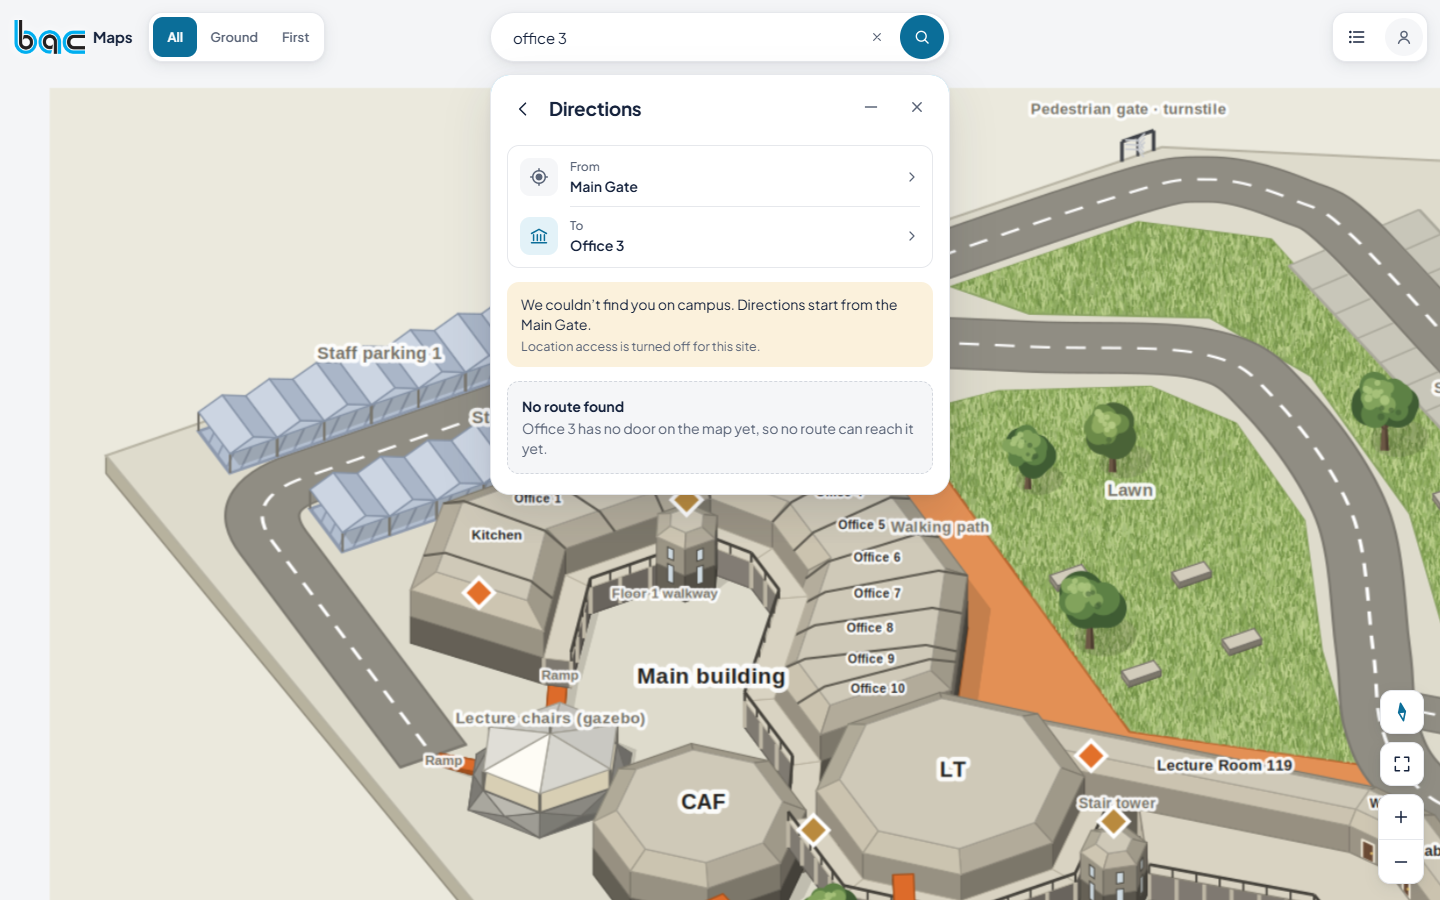
\includegraphics[width=\linewidth]{figures/tour/20-unreachable-room-honest-message.png}\caption{No route to Office 3 (FR-13)}\end{subfigure}
\caption{Directions: steps, alternative route, changed start and the no-route message}\label{fig:directions}
\end{figure}

\begin{figure}[htbp]
\centering
\begin{subfigure}{0.49\textwidth}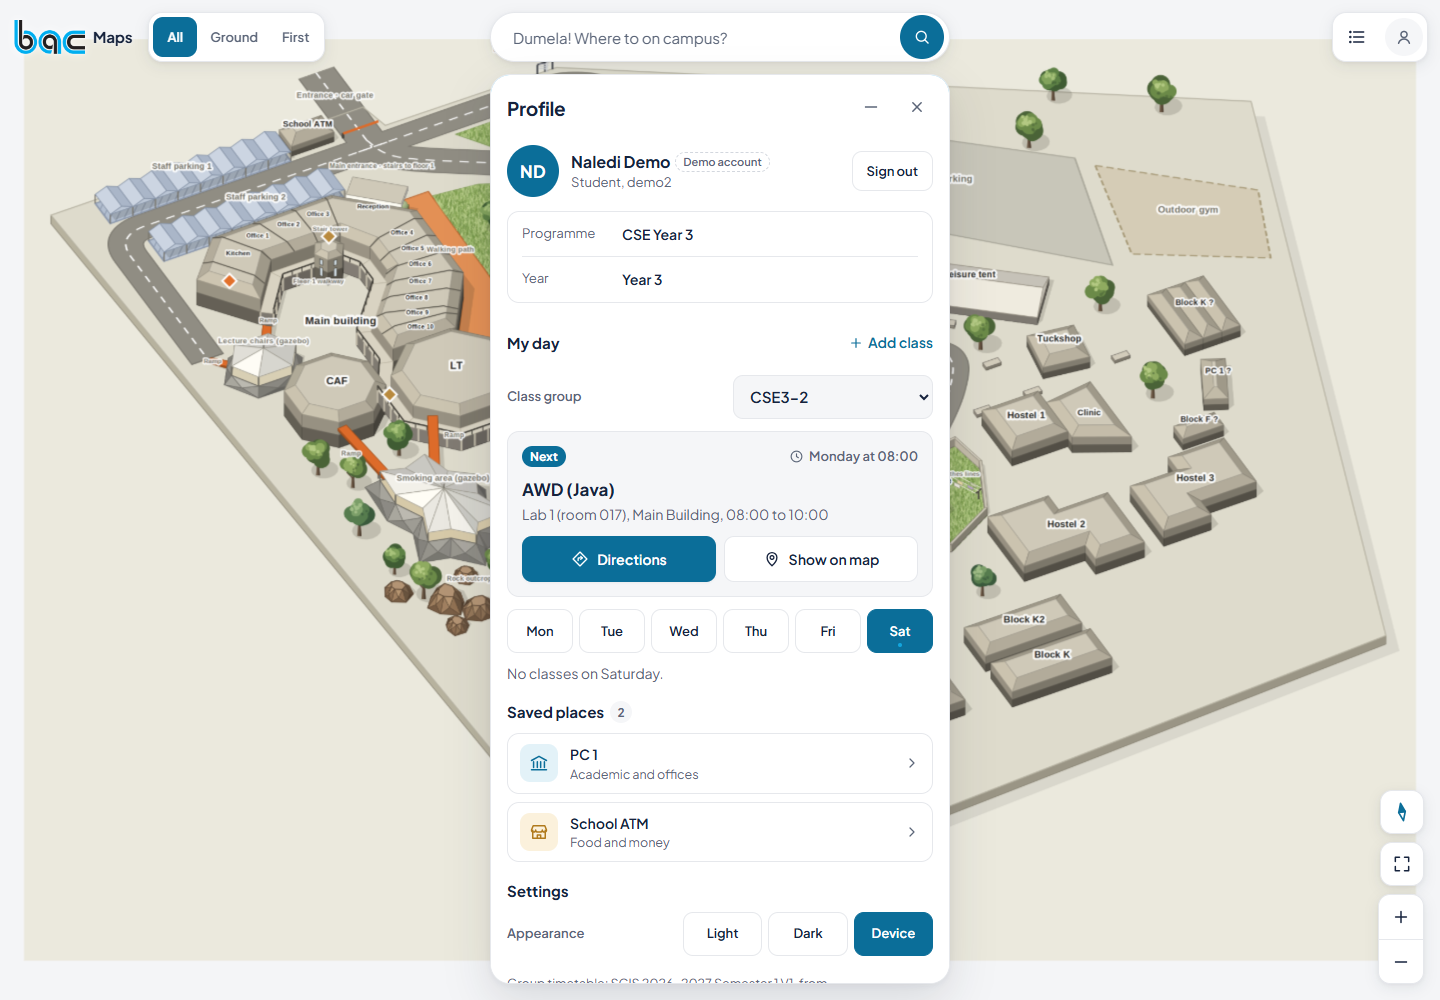
\includegraphics[width=\linewidth]{figures/tour/25-profile-timetable-light.png}\caption{Profile with group timetable (FR-16, FR-18)}\end{subfigure}\hfill
\begin{subfigure}{0.49\textwidth}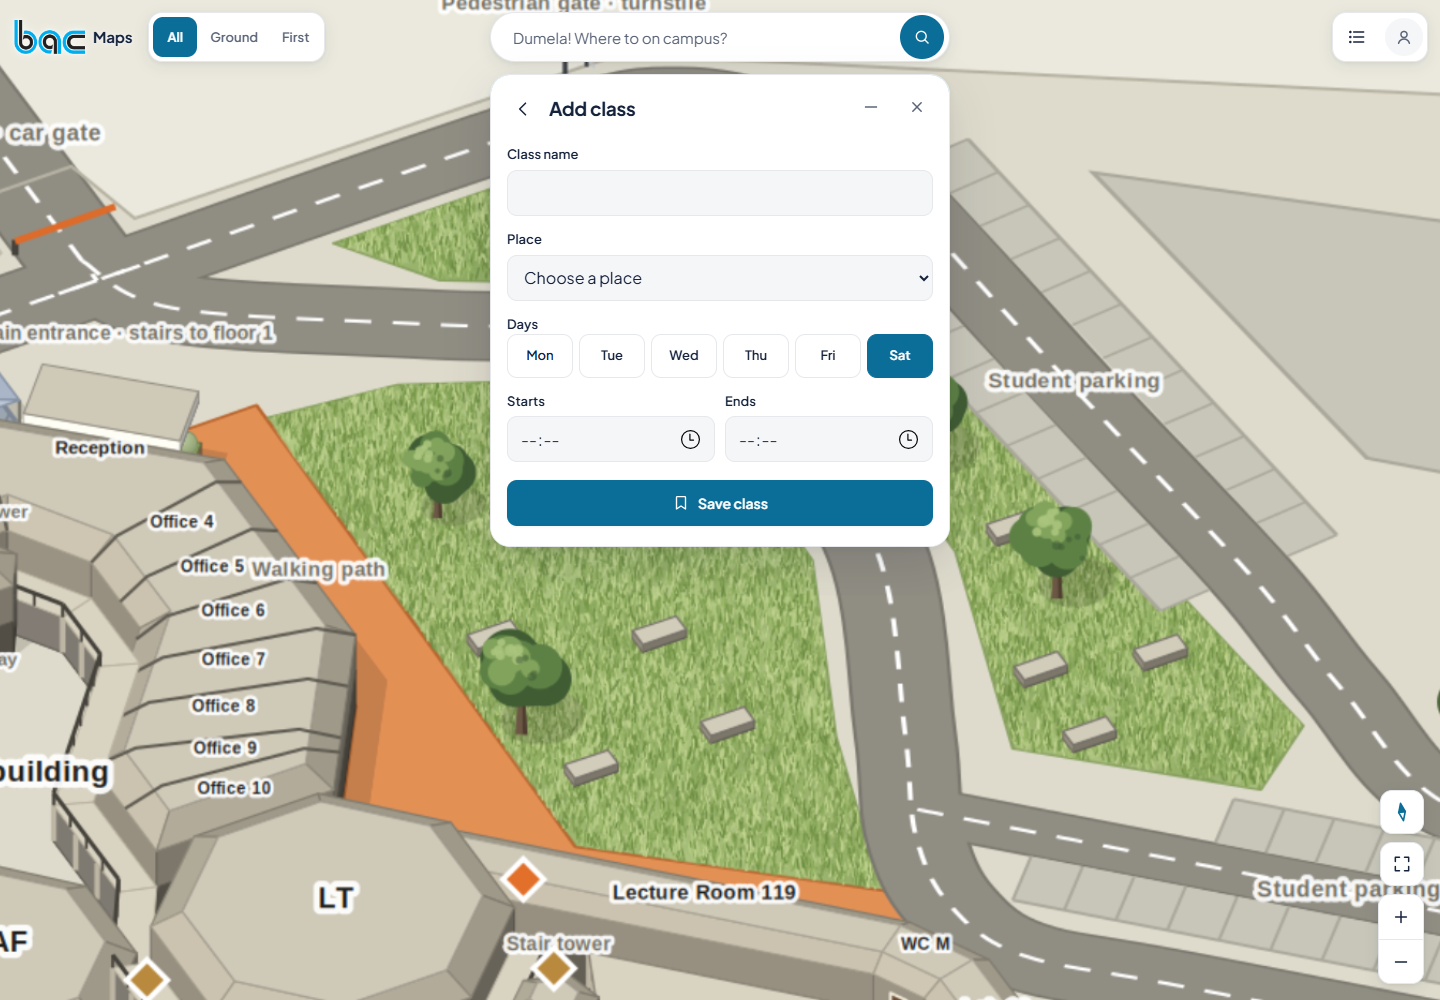
\includegraphics[width=\linewidth]{figures/tour/30-add-own-class-form.png}\caption{Adding an own class (FR-17)}\end{subfigure}\\[2mm]
\begin{subfigure}{0.49\textwidth}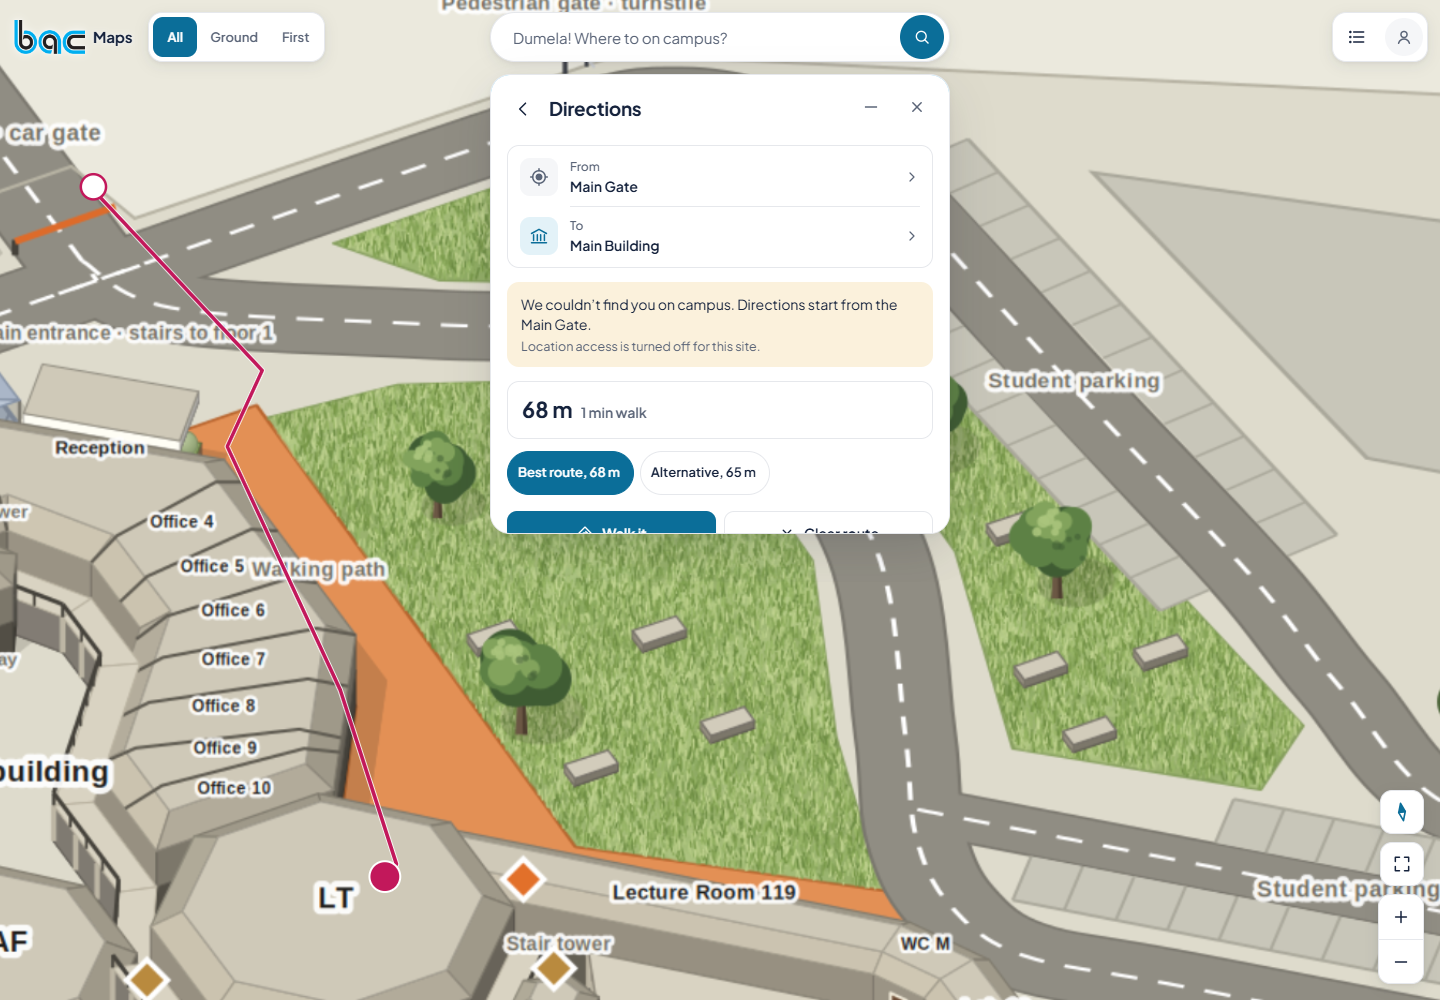
\includegraphics[width=\linewidth]{figures/tour/29-directions-to-class.png}\caption{Directions to a class (FR-18)}\end{subfigure}\hfill
\begin{subfigure}{0.49\textwidth}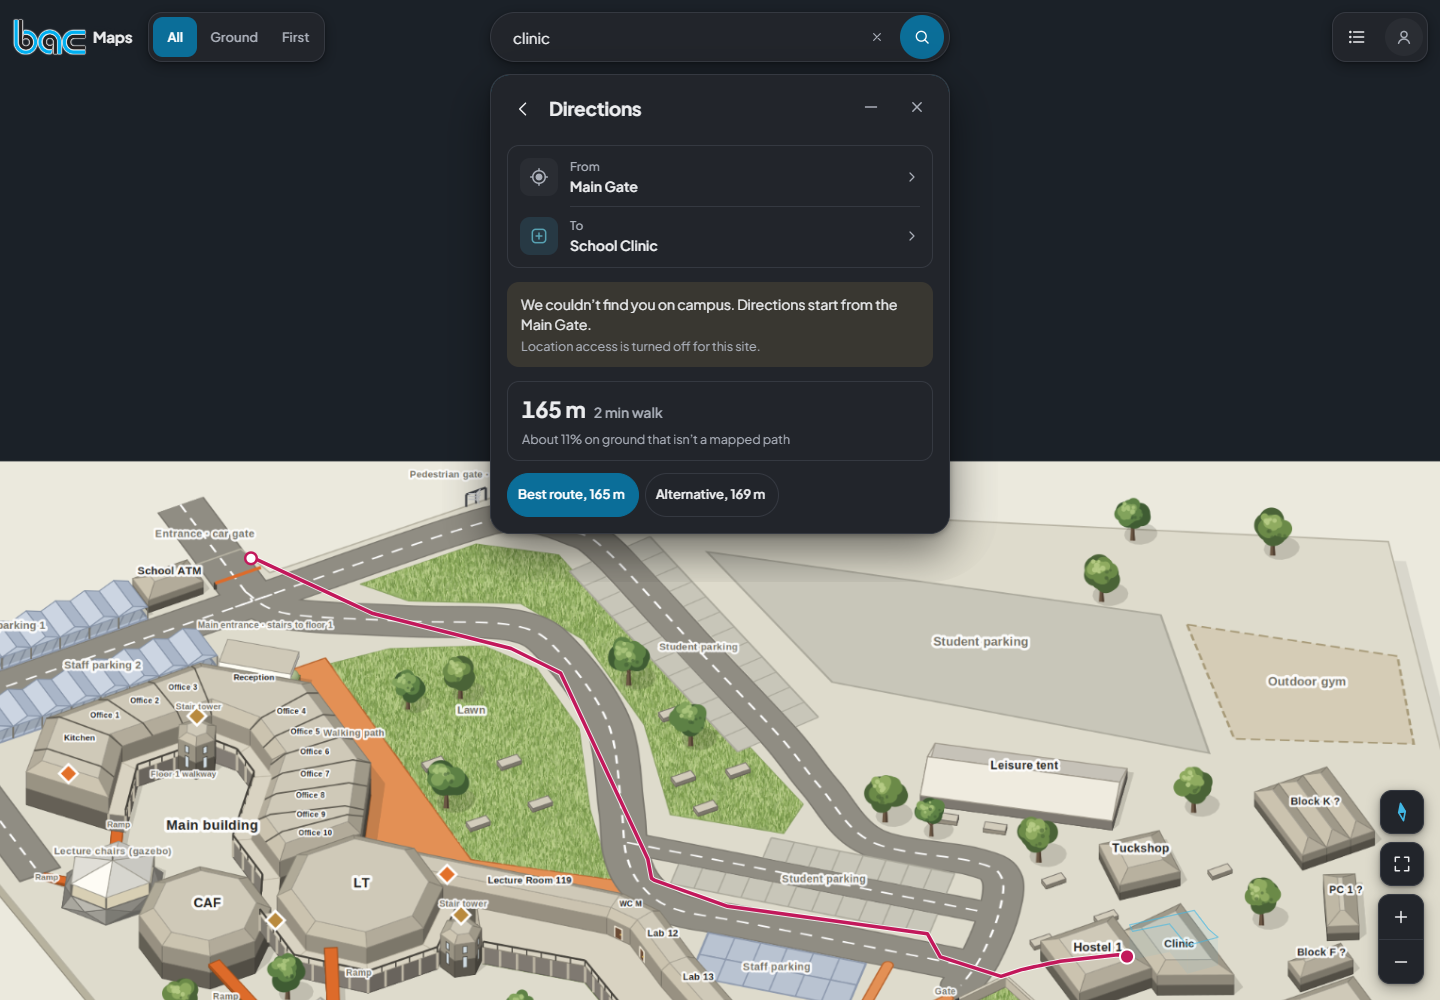
\includegraphics[width=\linewidth]{figures/tour/32-directions-dark-mode.png}\caption{Dark appearance (NFR-07)}\end{subfigure}
\caption{The profile, timetable and appearance settings}\label{fig:profile}
\end{figure}

\begin{figure}[htbp]
\centering
\begin{subfigure}{0.24\textwidth}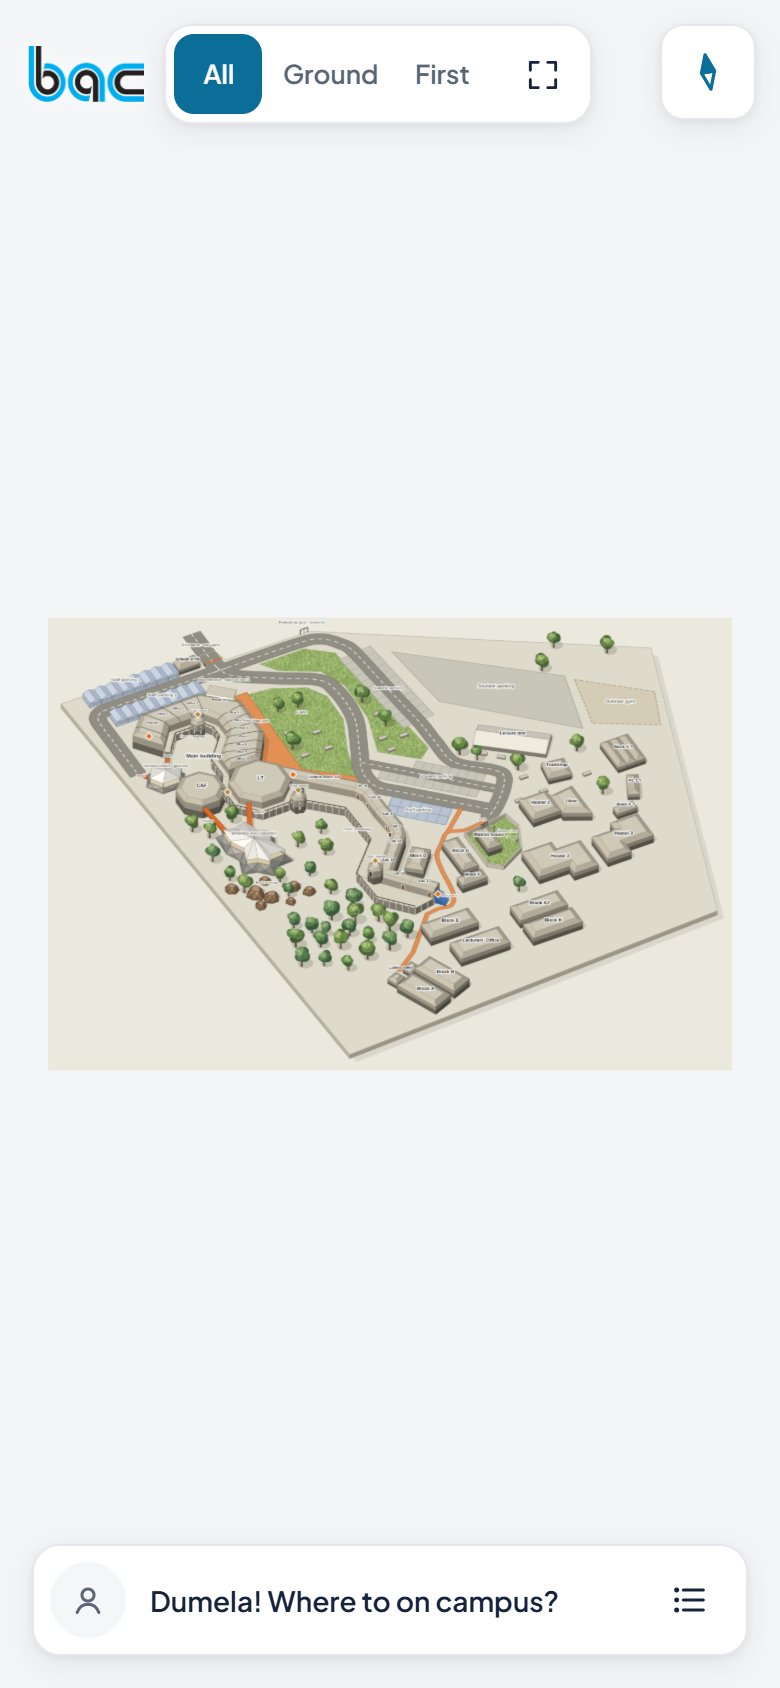
\includegraphics[width=\linewidth]{figures/tour/33-phone-home-pill.png}\caption{Home}\end{subfigure}\hfill
\begin{subfigure}{0.24\textwidth}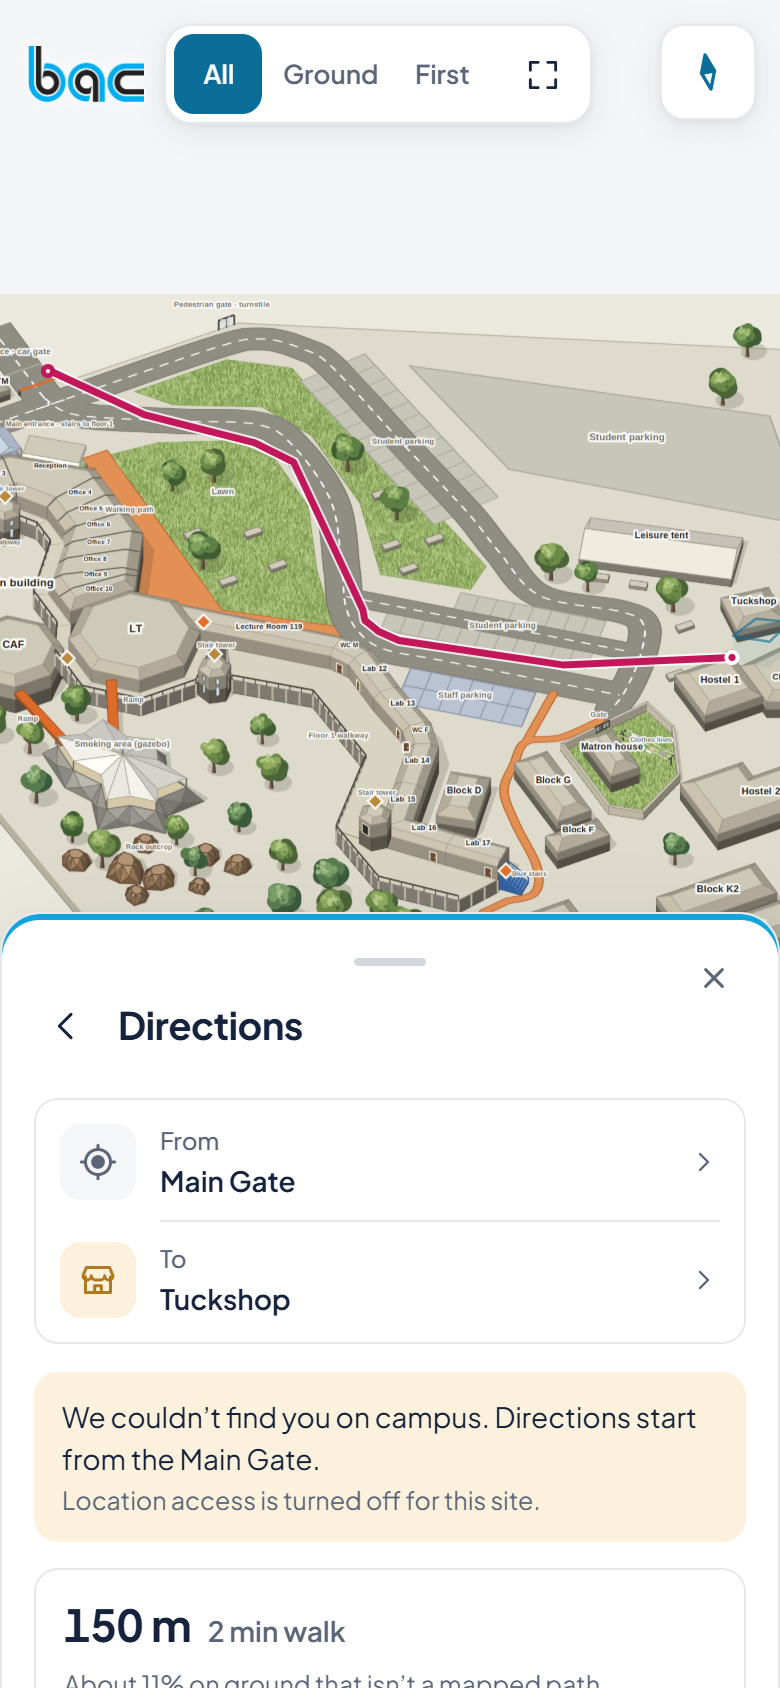
\includegraphics[width=\linewidth]{figures/tour/36-phone-directions.png}\caption{Directions}\end{subfigure}\hfill
\begin{subfigure}{0.24\textwidth}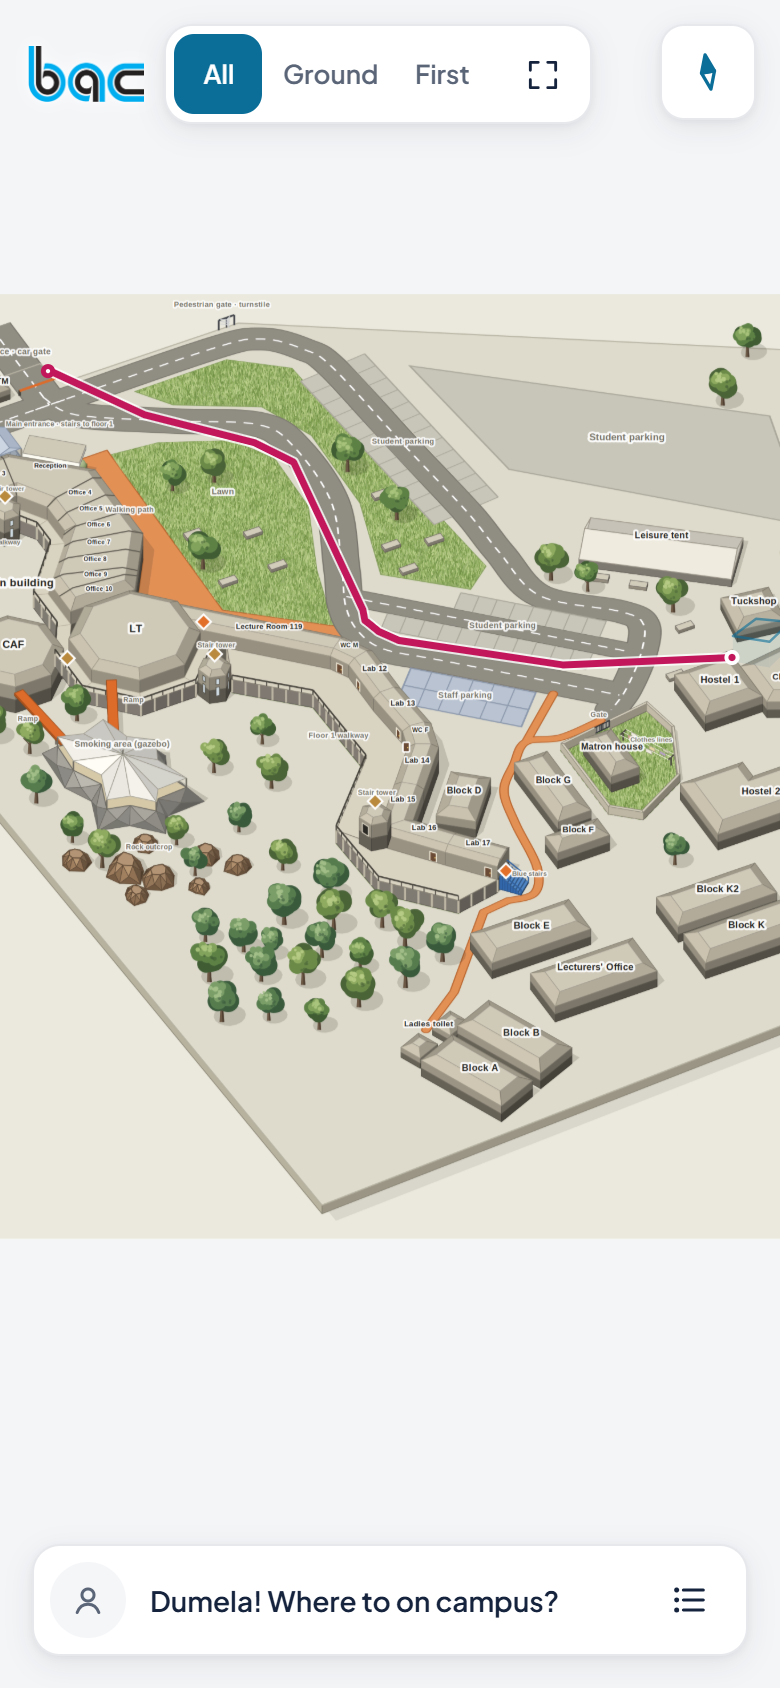
\includegraphics[width=\linewidth]{figures/tour/37-phone-route-full-map.png}\caption{Route on map}\end{subfigure}\hfill
\begin{subfigure}{0.24\textwidth}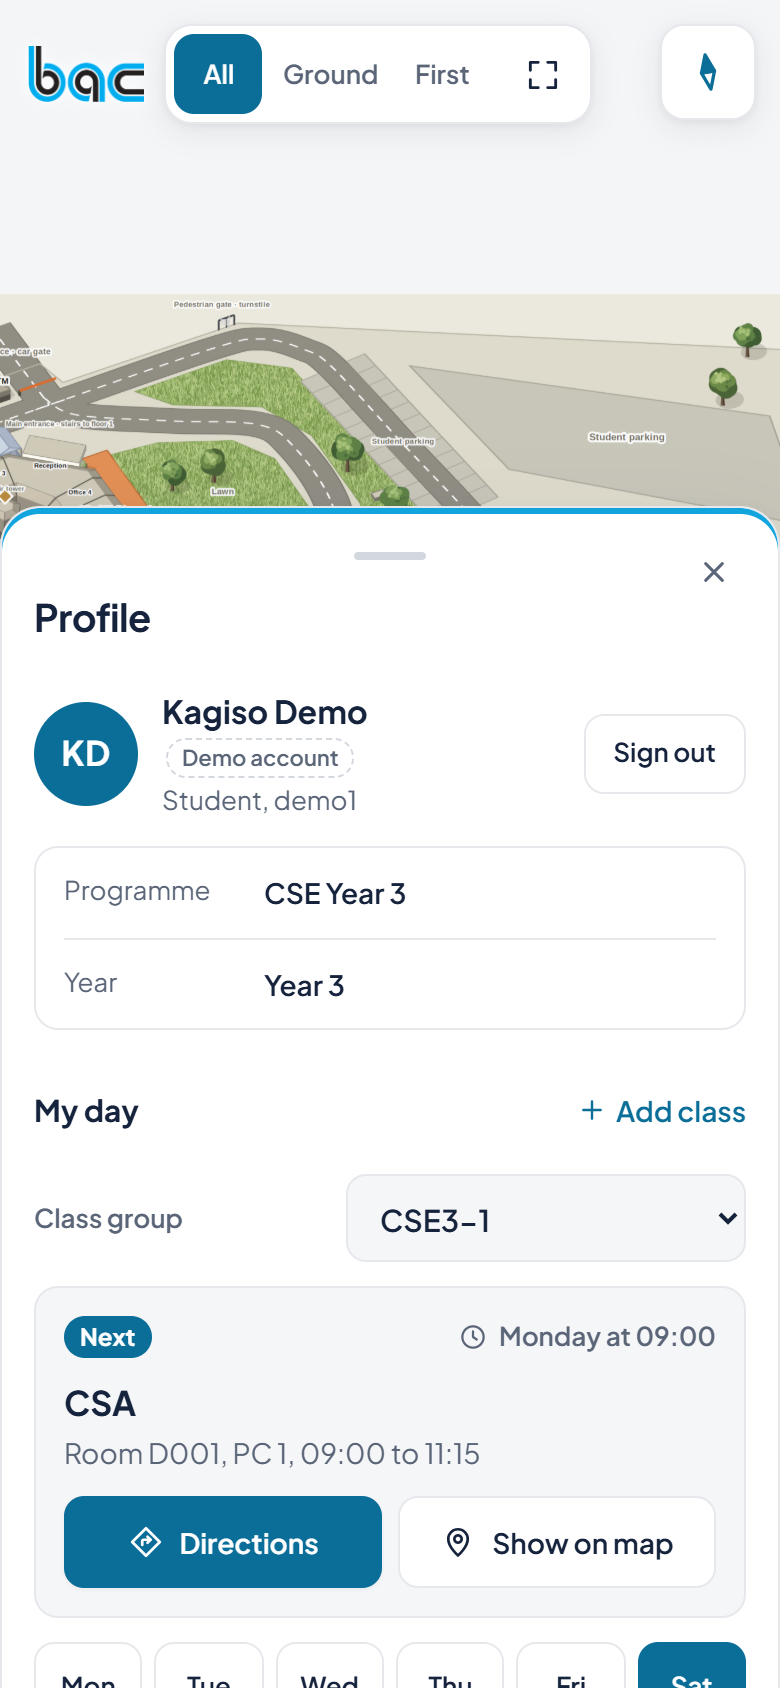
\includegraphics[width=\linewidth]{figures/tour/38-phone-profile-timetable.png}\caption{Timetable}\end{subfigure}
\caption{The application at phone size (390$\times$844, emulated in Microsoft Edge)}\label{fig:phone}
\end{figure}

\subsection{Change C1: BAC Maps joined to the finished map and Pathfinder}
Before this change, BAC Maps showed an approximate block map and its Directions panel only said that routes were coming (Figure~\ref{fig:c1}). The interface was connected to the campus drawings and to Pathfinder through the two adapters, so the map now shows the real campus, both floors and 40 rooms, and Directions returns real routes. Listing~\ref{lst:drawings} corrects the drawings' file paths, which was the first defect found (Table~\ref{tab:defects}, D1). Listing~\ref{lst:landmarks} finds the Main Gate and Student Entrance from the ends of the verified walks, because the traced data has no gate points.

\begin{figure}[htbp]
\centering
\begin{subfigure}{0.49\textwidth}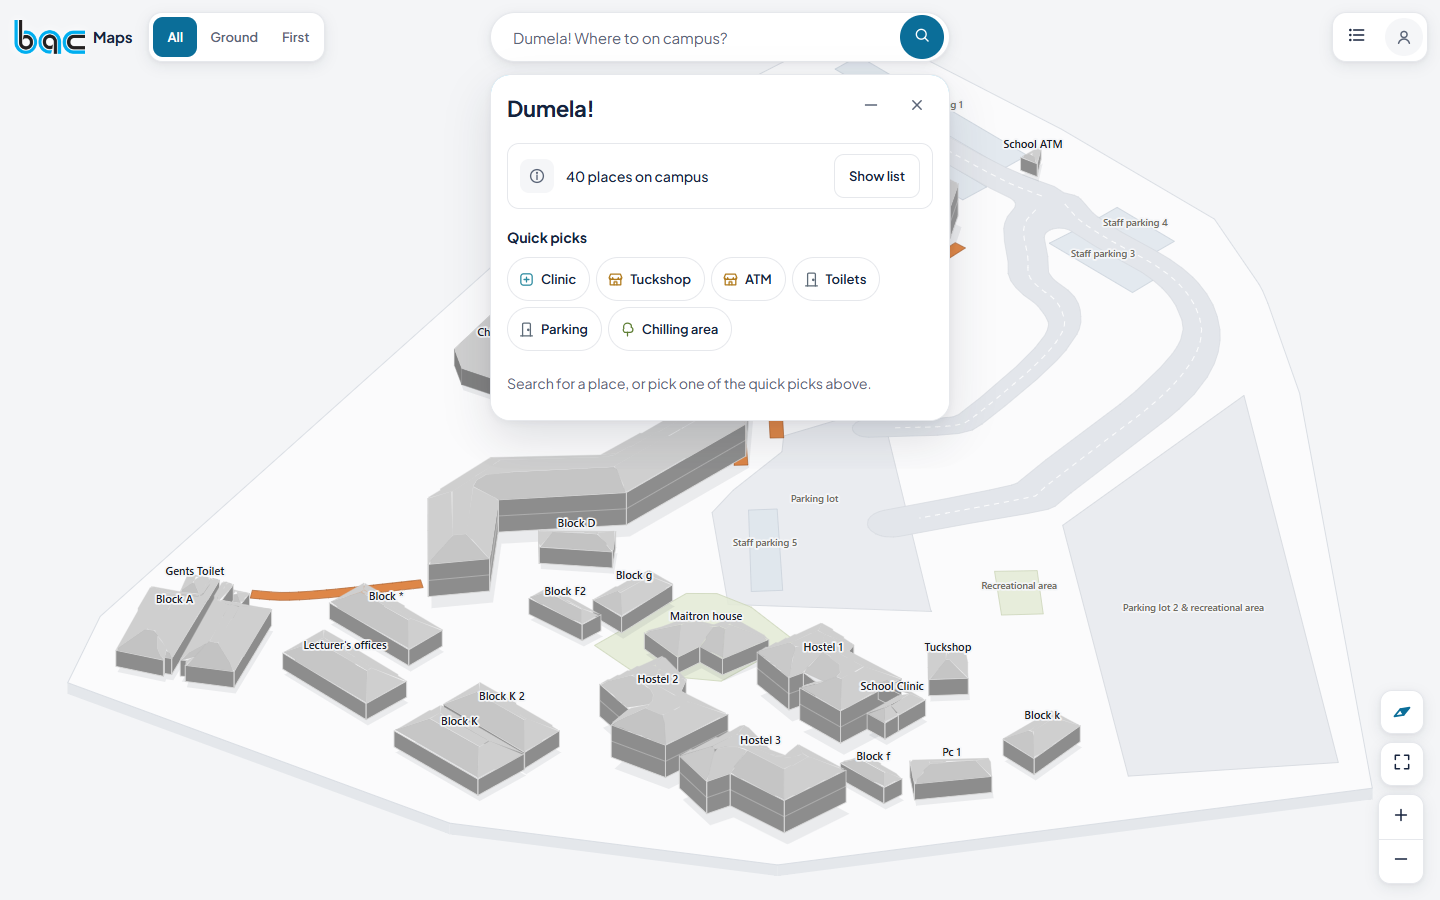
\includegraphics[width=\linewidth]{figures/before-c1-map.png}\caption{Before: approximate map}\end{subfigure}\hfill
\begin{subfigure}{0.49\textwidth}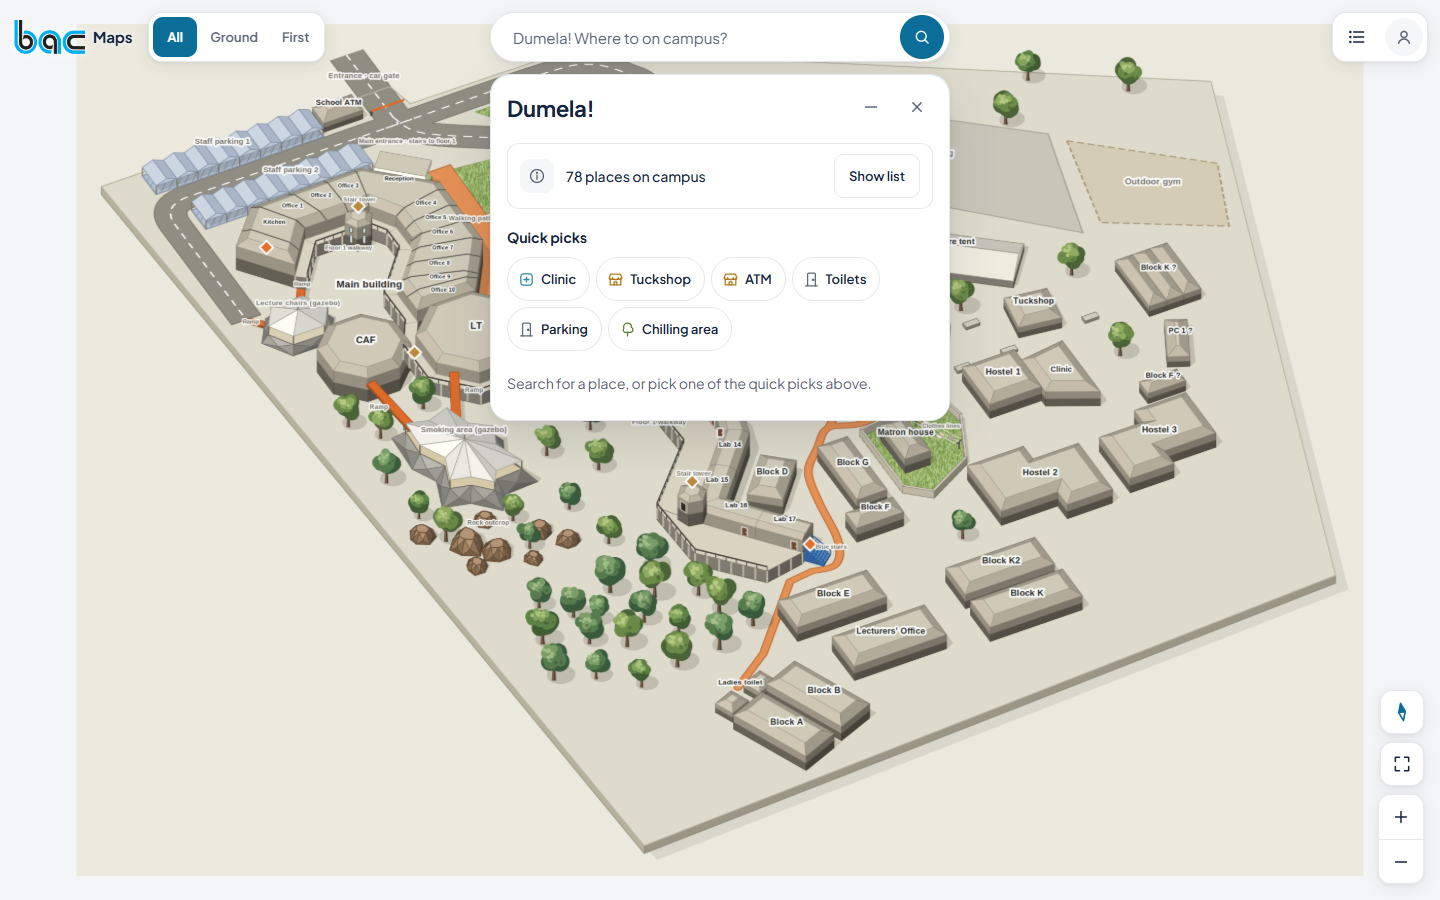
\includegraphics[width=\linewidth]{figures/tour/01-home-map-and-search-panel.png}\caption{After: the campus drawings}\end{subfigure}
\caption{C1, the map before and after joining the finished map}\label{fig:c1}
\end{figure}

\begin{figure}[htbp]
\centering
\begin{subfigure}{0.49\textwidth}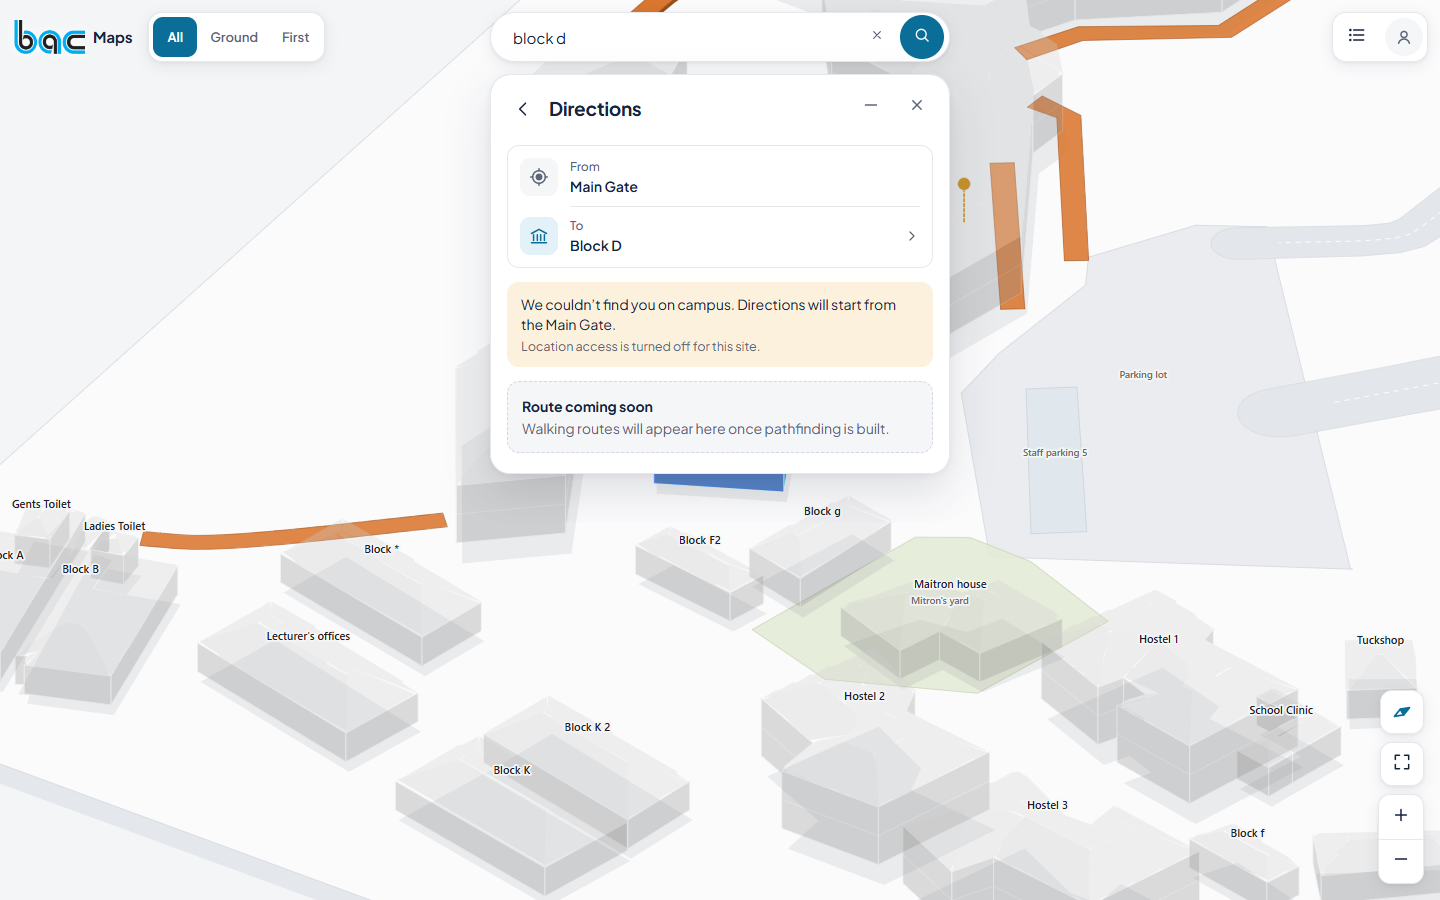
\includegraphics[width=\linewidth]{figures/before-c1-directions.png}\caption{Before: ``Route coming soon''}\end{subfigure}\hfill
\begin{subfigure}{0.49\textwidth}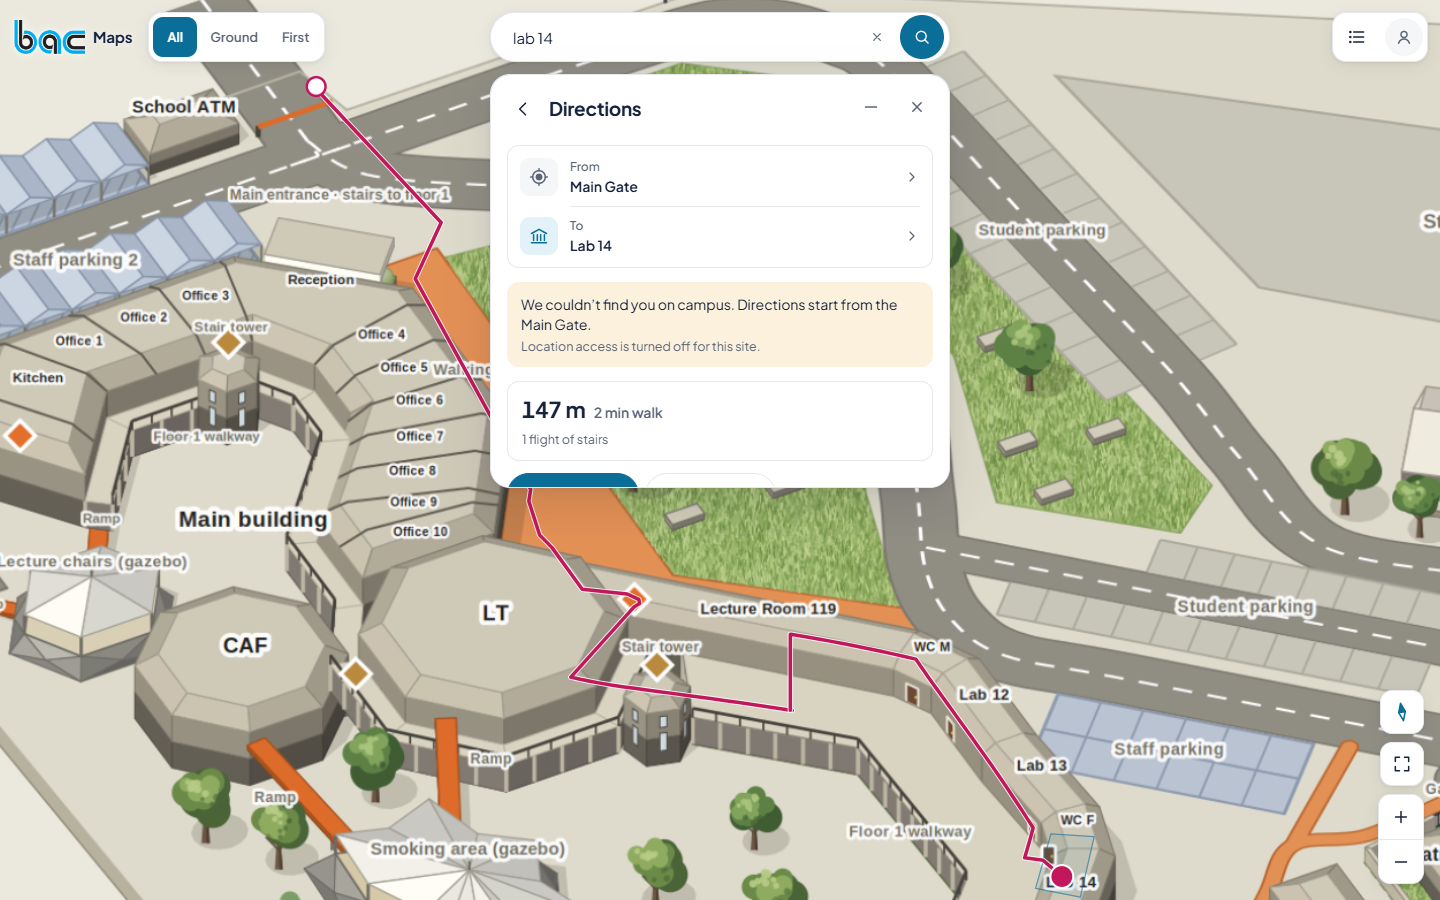
\includegraphics[width=\linewidth]{figures/tour/11-directions-pathfinder-route.png}\caption{After: a Pathfinder route to Lab 14}\end{subfigure}
\caption{C1, Directions before and after joining Pathfinder}\label{fig:c1-directions}
\end{figure}

\lstinputlisting[language=Java, firstline=64, lastline=71, caption={Correcting the drawings' paths for the website (frontend/src/lib/map-adapter.js, lines 64--71)}, label={lst:drawings}]{code/map-adapter.js}

\lstinputlisting[language=Java, firstline=51, lastline=66, caption={Finding the gates from the verified walks (frontend/src/lib/nav-adapter.js, lines 51--66)}, label={lst:landmarks}]{code/nav-adapter.js}

\subsection{The route-finding algorithm}\label{sec:algorithm}
Pathfinder builds a 0.5\,m grid of the campus outdoors and a graph of corridors, doors and stairs indoors. Walking on a traced path costs its length, on a verified walk 0.8 times its length, and on untraced open ground 2.5 times; a flight of stairs costs 10.4 and adds 12 seconds. The search expands nodes in order of
\begin{equation}\label{eq:astar}
  f(n) = g(n) + h(n), \qquad h(n) = 0.8 \cdot \min_{t \in T} \lVert \mathbf{x}_n - \mathbf{x}_t \rVert
\end{equation}
where $g(n)$ is the cost of the best path found to node $n$, $\mathbf{x}_n$ its position, $T$ the set of goal nodes and 0.8 the cost per metre of the cheapest surface. Because no surface is cheaper than 0.8, $h$ never overestimates and the route found is the cheapest \citep{hart1968}. Listing~\ref{lst:astar} shows the estimate and the edge relaxation. For the alternative route, nodes of the first route cost 2.2 times more, and a second search finds a route that differs from it. Searches run in 8\,ms slices so that the page never freezes, and every route is checked against walls every 25\,cm before it is shown.

\lstinputlisting[language=Java, firstline=694, lastline=703, caption={A* estimate and edge relaxation in Pathfinder (web/nav-engine.js, lines 694--703)}, label={lst:astar}]{code/nav-engine.js}

\subsection{Change C2: the timetable on the profile}
Before this change, the profile listed only classes the student had typed in, and students in older databases had no class group, so no timetable could be shown (Figure~\ref{fig:c2}). The profile now shows the student's class-group timetable by day, with the next class and directions to it, and loading, error and empty states. Listing~\ref{lst:groups} gives existing demonstration students their group when an older database is upgraded.

\begin{figure}[htbp]
\centering
\begin{subfigure}{0.49\textwidth}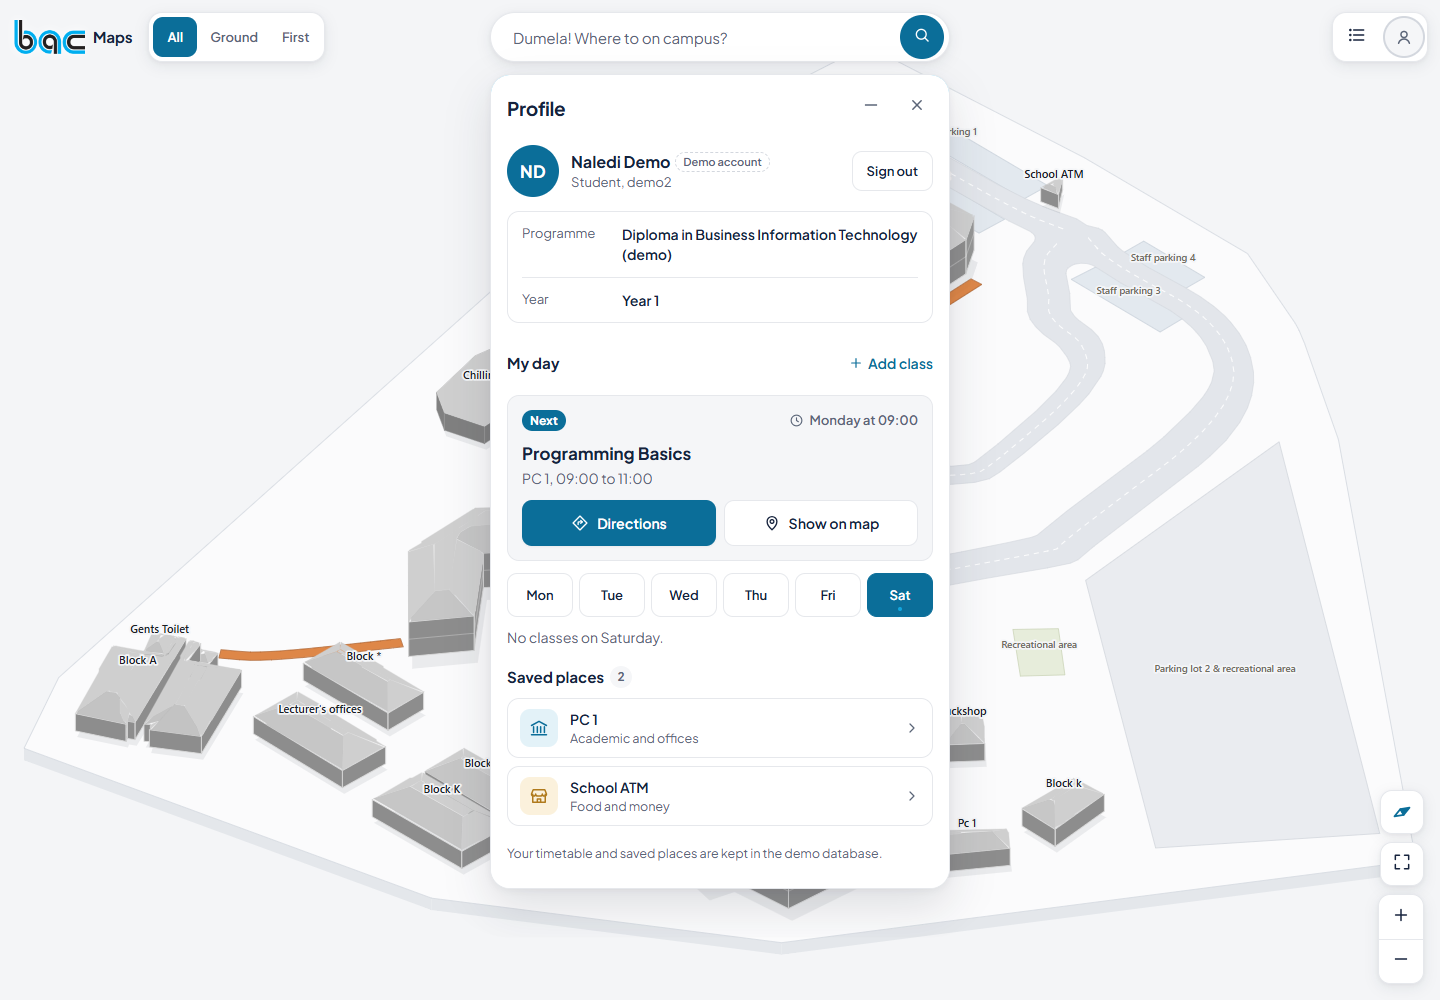
\includegraphics[width=\linewidth]{figures/before-c2-profile.png}\caption{Before: own classes only}\end{subfigure}\hfill
\begin{subfigure}{0.49\textwidth}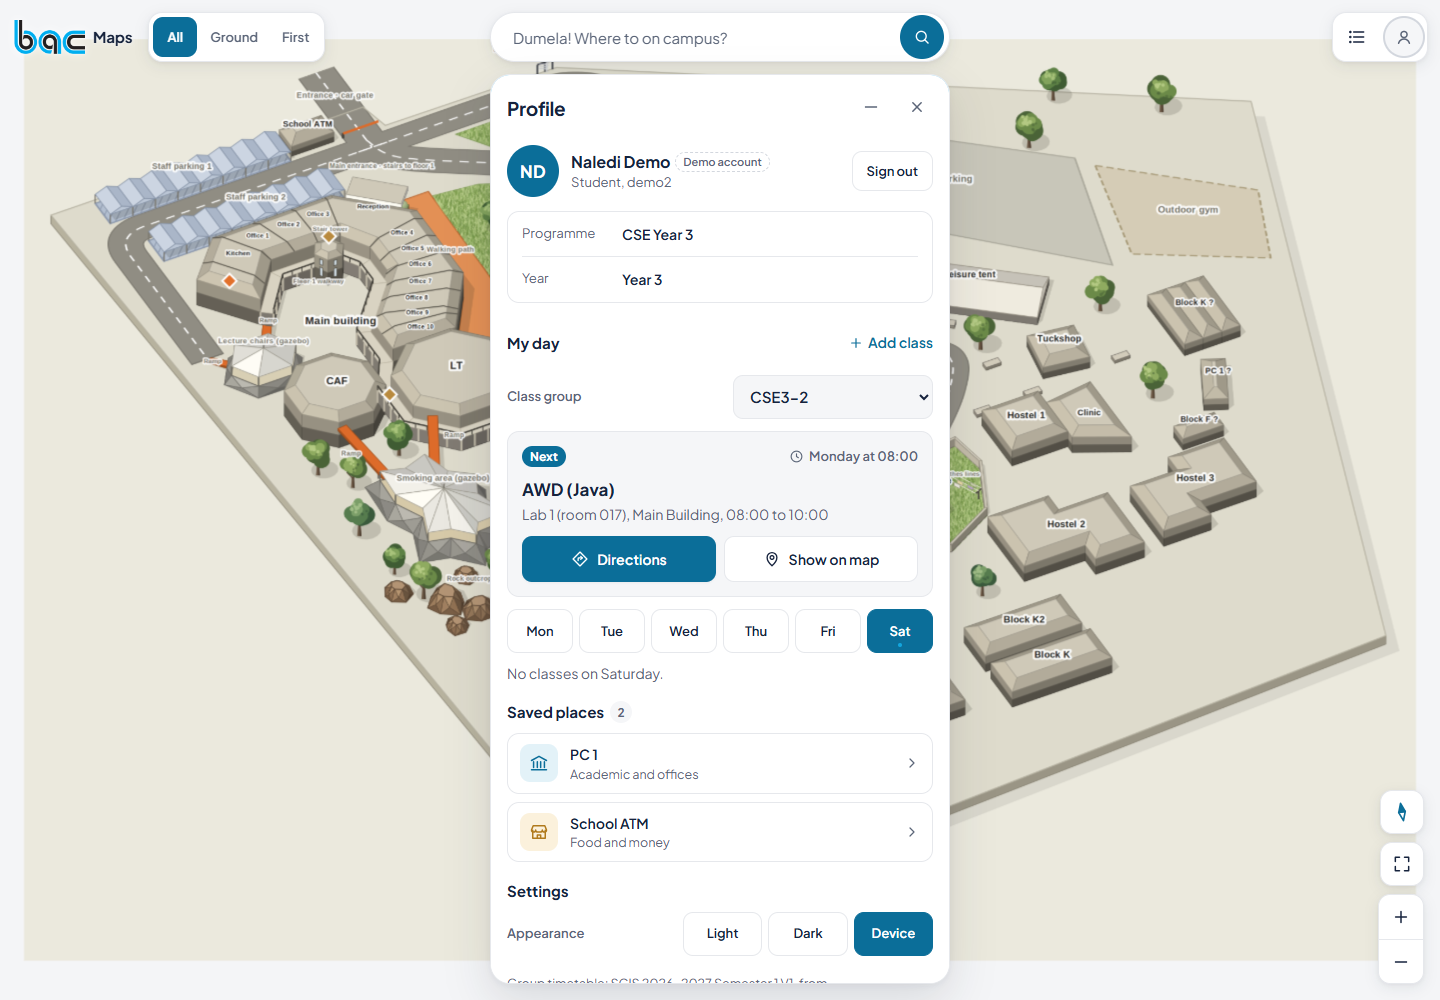
\includegraphics[width=\linewidth]{figures/after-c2-profile.png}\caption{After: group timetable}\end{subfigure}
\caption{C2, the profile before and after adding the class-group timetable}\label{fig:c2}
\end{figure}

\lstinputlisting[language=Python, firstline=83, lastline=89, caption={Upgrading an older database (server/db.py, lines 83--89)}, label={lst:groups}]{code/db.py}

\subsection{Change C3: routes kept clear of the panel}
Routes were centred on the screen, so on desktop the panel covered much of them, and on a phone the card covered the lower half of the map. The route is now placed in the largest free part of the map beside or below the panel (Listing~\ref{lst:free}), and the panel becomes shorter while a route is shown. The before image in Figure~\ref{fig:c3} was reproduced on the current build by switching this placement off, because the earlier build cannot show routes at all. The site suite measures that 100\% of the route is visible after the change on a phone.

\begin{figure}[htbp]
\centering
\begin{subfigure}{0.49\textwidth}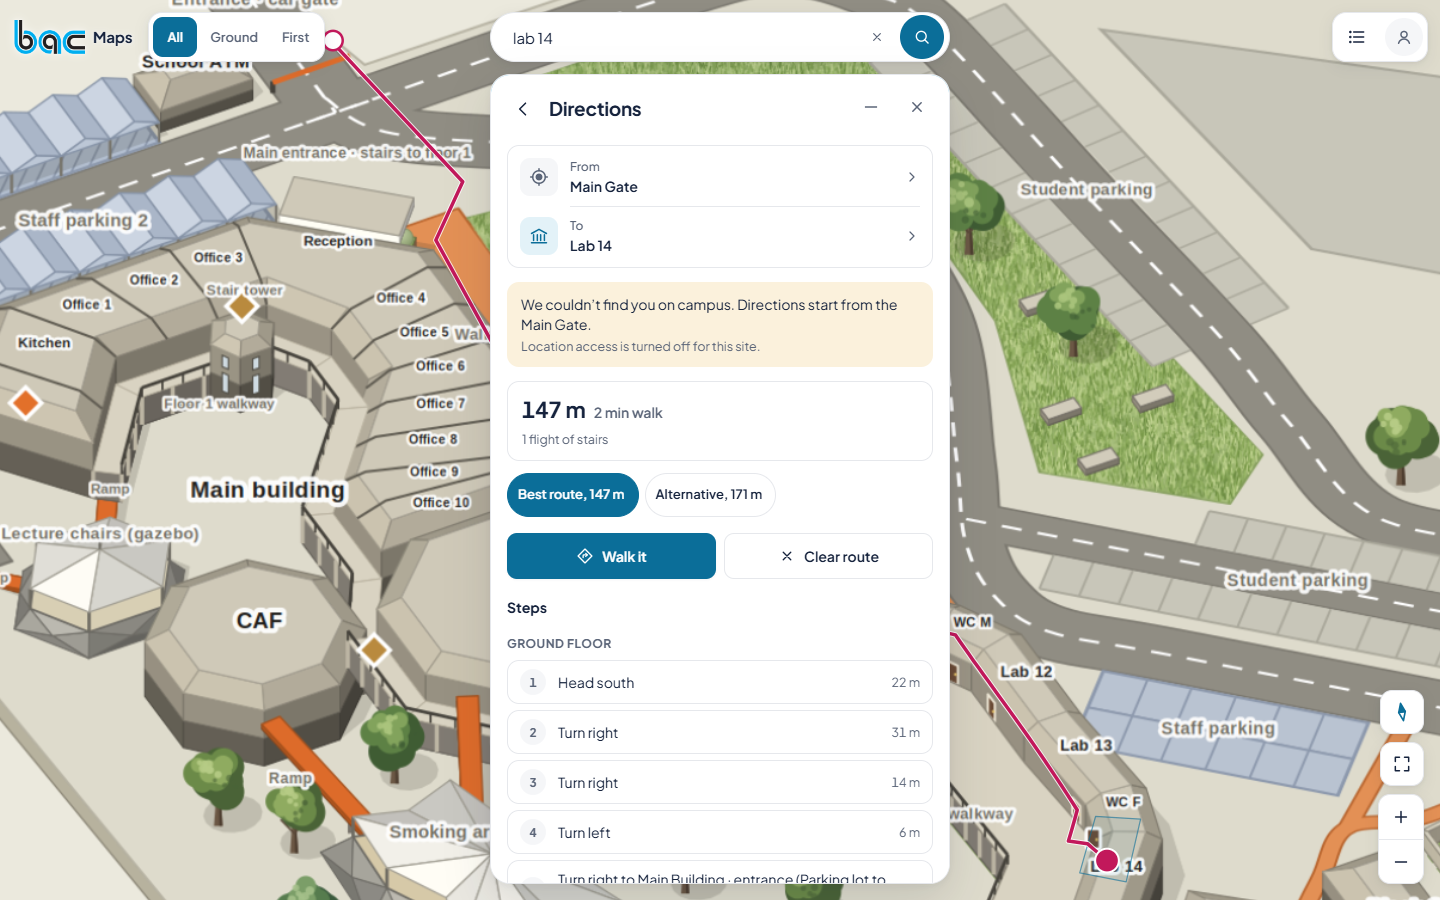
\includegraphics[width=\linewidth]{figures/before-c3-route-hidden.png}\caption{Before (reproduced): route under the panel}\end{subfigure}\hfill
\begin{subfigure}{0.49\textwidth}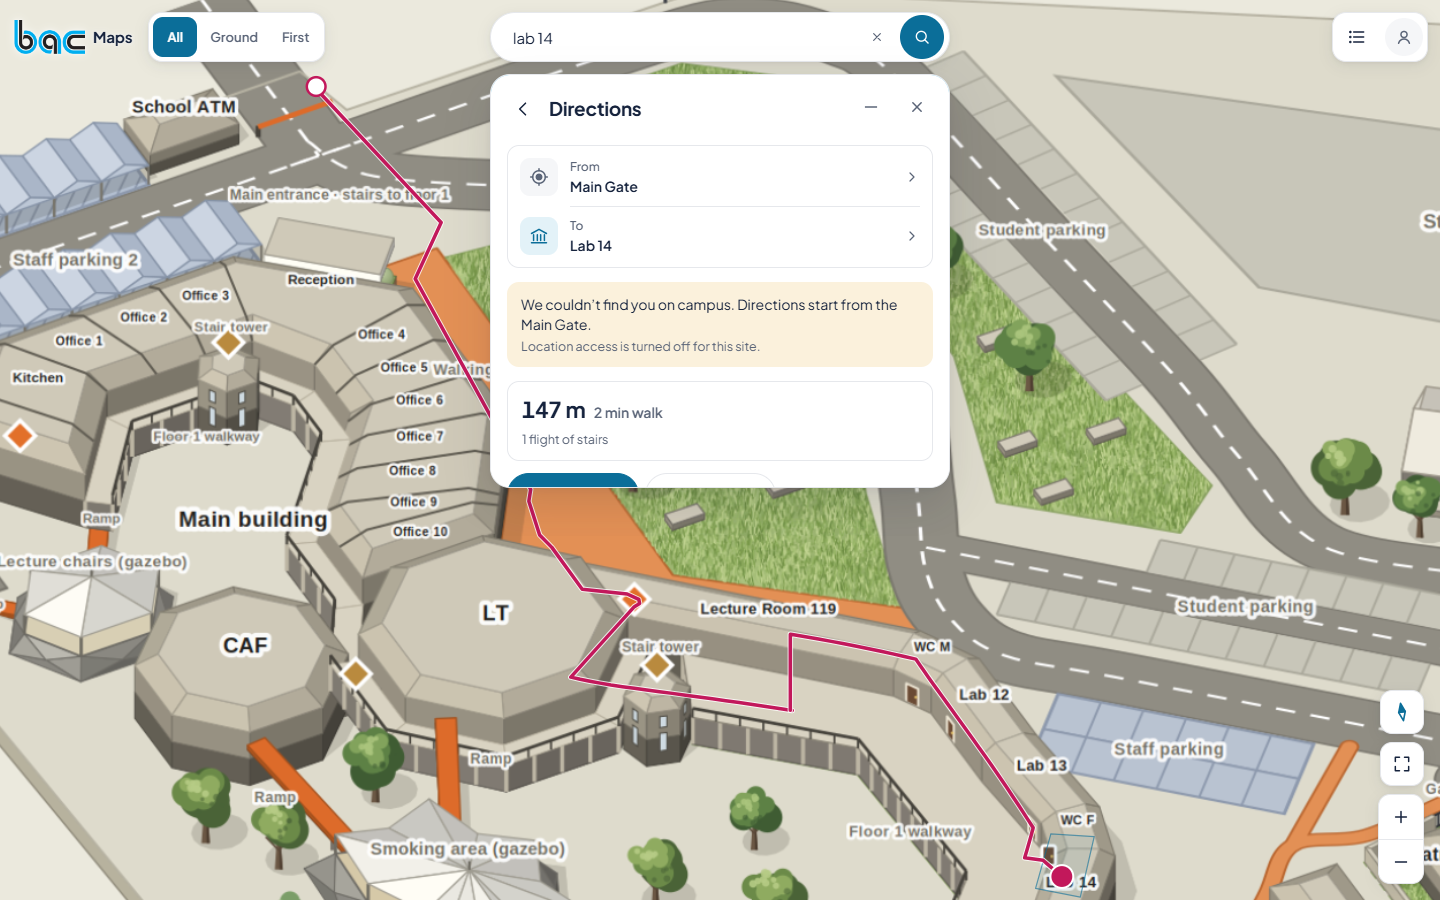
\includegraphics[width=\linewidth]{figures/after-c3-route-clear.png}\caption{After: route beside the panel}\end{subfigure}
\caption{C3, the route before and after placing it in the free part of the map}\label{fig:c3}
\end{figure}

\lstinputlisting[language=Java, firstline=73, lastline=89, caption={Free areas of the map around the panel (frontend/src/components/App.jsx, lines 73--89)}, label={lst:free}]{code/App.jsx}

\subsection{Change C4: the interface rebuilt in React}
The interface was rewritten from one 1\,557-line script that built every view with DOM calls into React components built with Vite (Figure~\ref{fig:structure}). The map, Pathfinder and their adapters keep the same logic, and the interface looks the same, so no before-and-after screenshot is given. The build writes its file names into the service worker, which now caches 26 files under version~9. Three defects appeared while porting and were fixed before release: an extra wrapper around icons broke their styling, the start picker's header and list did not share state, and the view stack hid views during their slide animation.

\begin{figure}[htbp]
\centering
\resizebox{0.95\textwidth}{!}{% C4: structure of the interface code before and after the React rebuild
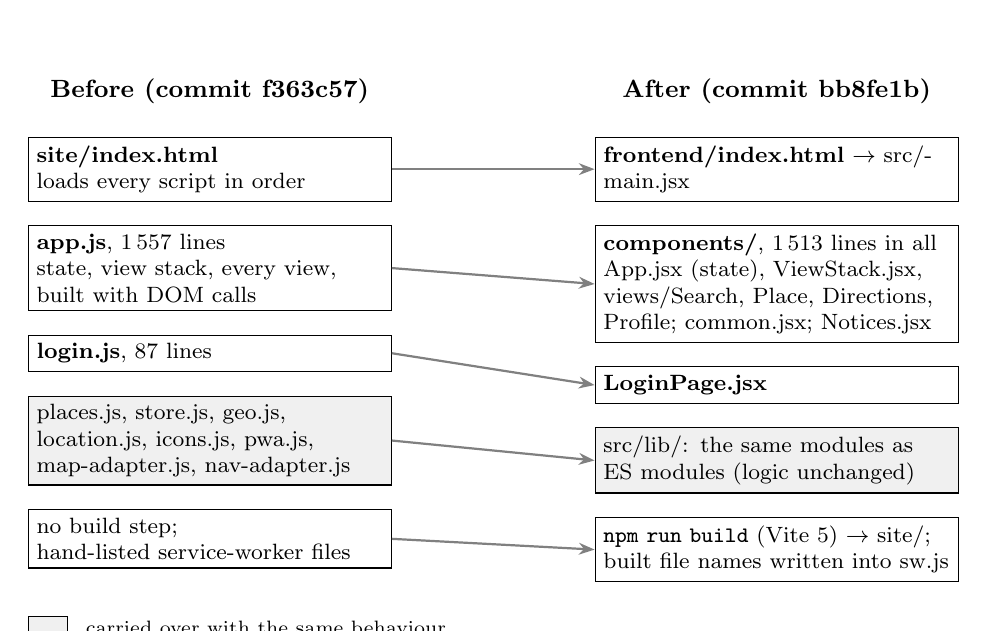
\begin{tikzpicture}[
  font=\footnotesize, node distance=3mm,
  f/.style={draw, align=left, minimum width=46mm, inner sep=3pt, fill=white, text width=44mm},
  same/.style={f, fill=gray!12},
  arr/.style={-{Stealth[length=2mm]}, thick}]

  \node[font=\small\bfseries] (bt) at (0,0) {Before (commit f363c57)};
  \node[f, below=of bt] (b1) {\textbf{site/index.html}\\ loads every script in order};
  \node[f, below=of b1] (b2) {\textbf{app.js}, 1\,557 lines\\ state, view stack, every view, built with DOM calls};
  \node[f, below=of b2] (b3) {\textbf{login.js}, 87 lines};
  \node[same, below=of b3] (b4) {places.js, store.js, geo.js,\\ location.js, icons.js, pwa.js,\\ map-adapter.js, nav-adapter.js};
  \node[f, below=of b4] (b5) {no build step;\\ hand-listed service-worker files};

  \node[font=\small\bfseries] (at) at (7.2,0) {After (commit bb8fe1b)};
  \node[f, below=of at] (a1) {\textbf{frontend/index.html} $\rightarrow$ src/main.jsx};
  \node[f, below=of a1] (a2) {\textbf{components/}, 1\,513 lines in all\\ App.jsx (state), ViewStack.jsx,\\ views/Search, Place, Directions,\\ Profile; common.jsx; Notices.jsx};
  \node[f, below=of a2] (a3) {\textbf{LoginPage.jsx}};
  \node[same, below=of a3] (a4) {src/lib/: the same modules as\\ ES modules (logic unchanged)};
  \node[f, below=of a4] (a5) {\texttt{npm run build} (Vite 5) $\rightarrow$ site/;\\ built file names written into sw.js};

  \foreach \i in {1,...,5} \draw[arr, gray] (b\i.east) -- (a\i.west);
  \node[draw, fill=gray!12, minimum width=5mm, minimum height=3mm, below=6mm of b5.south west, anchor=north west] (k) {};
  \node[right=1mm of k, font=\scriptsize] {carried over with the same behaviour};
\end{tikzpicture}
}
\caption{C4, structure of the interface code before and after the React rebuild}\label{fig:structure}
\end{figure}

\subsection{Change C5: defects found in testing and fixed}
Table~\ref{tab:defects} lists the ten defects found while testing the merged application, with their causes and corrections.

\begin{table}[htbp]
\centering\tablespacing
\caption{Defects found in testing and fixed}\label{tab:defects}
\begin{tabular}{p{0.7cm}p{4.4cm}p{4.2cm}p{4.4cm}}
\toprule
No. & Observed problem & Cause & Correction \\
\midrule
D1 & The campus drawings did not load & Image paths pointed to the wrong folder & The map adapter corrects the paths \\
D2 & The timetable was missing from the profile & The timetable work had never been merged in & Merged in, file by file \\
D3 & Existing students still had no timetable & Upgrading the database left their group empty & Demo students receive their group on upgrade \\
D4 & A signed-in student briefly appeared as a guest & The profile had no loading state & Loading, error and empty states added \\
D5 & No routes in a background tab & Pathfinder waited for the screen to redraw & A timer now starts it as well \\
D6 & The walking marker stayed after Clear route & Its clean-up was lost when the walk ended & Clean-up kept until the route is cleared \\
D7 & The top search showed the previous results & The search view wrote the old text back & The new text is kept first \\
D8 & Routes hidden behind the panel & Routes were centred on the screen & Placed in the free part of the map (C3) \\
D9 & A route partly covered once the panel filled & Placed while the panel was still loading & Placed after the panel is drawn \\
D10 & Outdated files appeared during testing & The offline cache kept serving them & Cache version raised; cache cleared between runs \\
\bottomrule
\end{tabular}
\end{table}

\subsection{Test results}
All suites were run on 24 October 2026 on Windows~11 with Node.js 24.14.1, Python 3.12.10 and Microsoft Edge 155 (headless, through Playwright), against commit \texttt{bb8fe1b}. Table~\ref{tab:suites} gives the results. Phone results come from Edge at a phone size of 390$\times$844 with touch emulation, not from a real phone.

\begin{table}[htbp]
\centering\tablespacing
\caption{Automated test suites, 24 October 2026}\label{tab:suites}
\begin{tabular}{p{3.2cm}p{7.3cm}r r}
\toprule
Suite & What it checks & Passed & Failed \\
\midrule
nav & grid, movement, routes outdoors & 29 & 0 \\
interiors & rooms, doors, stairs; no route through a wall & 29 & 0 \\
scenarios & demonstration routes, every position on walkable ground & 24 & 0 \\
walks & 91 routes, none crossing a wall or leaving walkable ground & 66 & 0 \\
concurrency & overlapping and cancelled searches & 2 & 0 \\
e2e\_site & search, directions, route visibility, button sizes, no script errors & 35 & 0 \\
e2e\_profile & guest and signed-in profile, group timetable, loading and error states, next class & 40 & 0 \\
e2e\_floors & Pathfinder page (same engine and data): floor controls; 1\,482 routes checked against walls & 22 & 0 \\
\midrule
Total & & 247 & 0 \\
\bottomrule
\end{tabular}
\end{table}

Two older suites for the separate Pathfinder demonstration page (\texttt{e2e\_core}, \texttt{e2e\_perf}) do not complete: \texttt{e2e\_core} passed 21 checks, failed 4 and then stopped. The same four failures occur on the commit before the merge (\texttt{fafb968}), so they come from that page's tests, not from this version's changes (Section~\ref{sec:unexpected}).

Table~\ref{tab:cases} maps test cases to the requirements, and Table~\ref{tab:timings} gives the timings. Table~\ref{tab:security} gives the security checks.

{\tablespacing
\begin{longtable}{p{0.9cm}>{\raggedright}p{6.3cm}>{\raggedright}p{1.4cm}>{\raggedright}p{3.4cm}>{\raggedright\arraybackslash}p{1.3cm}}
\caption{Test cases and results}\label{tab:cases}\\
\toprule
ID & Test & Req. & Evidence & Result \\
\midrule\endfirsthead
\toprule
ID & Test & Req. & Evidence & Result \\
\midrule\endhead
\bottomrule\endfoot
T-01 & Map shows the campus drawings; zoom, pan and reset work & FR-01 & e2e\_site & Pass \\
T-02 & All, Ground and First change the floor without reloading & FR-02 & e2e\_site, e2e\_floors & Pass \\
T-03 & Searching ``first floor lab'' lists the six first-floor labs & FR-03 & e2e\_site & Pass \\
T-04 & Category chips and directory list the right places & FR-04 & manual & Pass \\
T-05 & Tapping a building opens its card & FR-05 & e2e\_site & Pass \\
T-06 & Room card shows category, building and floor & FR-06 & e2e\_site & Pass \\
T-07 & Route from the Main Gate to Lab 14 is found and drawn & FR-07 & e2e\_site & Pass \\
T-08 & Route uses stairs; steps grouped by floor & FR-08 & e2e\_site, scenarios & Pass \\
T-09 & No route sample crosses a wall (1\,482 routes; 91 walk routes) & FR-08 & e2e\_floors, walks & Pass \\
T-10 & Alternative route offered and selectable & FR-09 & e2e\_site & Pass \\
T-11 & Changing start and destination recalculates & FR-10 & e2e\_site & Pass \\
T-12 & With location blocked, the route starts at the Main Gate & FR-11 & e2e\_site & Pass \\
T-13 & Position on campus used as the start (real phone) & FR-11 & -- & Not tested \\
T-14 & Walk it animates the marker; Clear route removes it & FR-12 & e2e\_site & Pass \\
T-15 & Office 3 gives a reason instead of a route & FR-13 & e2e\_site & Pass \\
T-16 & 100\% of the route visible beside the panel on a phone & FR-14 & e2e\_site & Pass \\
T-17 & Sign-in, sign-out; wrong password refused & FR-15 & e2e\_profile, Table~\ref{tab:security} & Pass \\
T-18 & Group timetable shown by day, with loading and error states & FR-16 & e2e\_profile & Pass \\
T-19 & Add, edit and delete an own class; invalid times refused & FR-17 & manual, Table~\ref{tab:security} & Pass \\
T-20 & Next class card with directions & FR-18 & e2e\_profile & Pass \\
T-21 & Save and unsave a place & FR-19 & manual & Pass \\
T-22 & Staff edits saved and used by routes (Pathfinder page) & FR-20 & manual & Partly \\
T-23 & Response times within 2 s & NFR-01 & Table~\ref{tab:timings} & Partly \\
T-24 & Another account cannot read or change a class & NFR-04 & Table~\ref{tab:security} & Pass \\
T-25 & Every visible button at least 44\,px tall & NFR-07 & e2e\_site, e2e\_profile & Pass \\
T-26 & Map and route work offline after one visit & NFR-10 & Section~\ref{sec:offline} & Pass \\
T-27 & Installation on a phone & NFR-10 & -- & Not tested \\
\end{longtable}}

\begin{table}[htbp]
\centering\tablespacing
\caption{Response times in milliseconds (median of five runs, range in brackets)}\label{tab:timings}
\begin{tabular}{p{4.2cm}p{4.6cm}p{4.6cm}}
\toprule
Measurement & Local server & 4G-like network, 4$\times$ slower processor \\
\midrule
Map ready (first visit) & 1\,394 (1\,152--2\,072) & 3\,439 (3\,412--4\,689) \\
Switch to ground floor & 16 (10--22) & 38 (31--48) \\
Switch to first floor & 42 (24--95) & 65 (49--93) \\
Route to Lab 14 shown & 93 (86--129) & 484 (450--546) \\
Data transferred & 2\,468\,kB & 2\,495\,kB \\
\bottomrule
\end{tabular}
\end{table}

\begin{table}[htbp]
\centering\tablespacing
\caption{Security checks against the demonstration server}\label{tab:security}
\begin{tabular}{>{\raggedright}p{8.2cm}>{\raggedright}p{3.6cm}>{\raggedright\arraybackslash}p{1.4cm}}
\toprule
Check & Response & Result \\
\midrule
Sign-in with a wrong password, or an unknown number & 401 & Pass \\
Reading classes without a session, or after signing out & 401 & Pass \\
Second account lists classes: first account's class absent & not listed & Pass \\
Second account edits the first account's class & 404 & Pass \\
Second account deletes it: still present for its owner & still present & Pass \\
Invalid group or a class that ends before it starts & 400 & Pass \\
Session cookie flags & HttpOnly, SameSite=Strict & Pass \\
Database, seed file, Git config, raw timetable, build scripts, a path climbing out of \texttt{/site/} & 404 & Pass \\
\bottomrule
\end{tabular}
\end{table}

\subsection{Offline behaviour}\label{sec:offline}
After one visit with the service worker enabled, the browser held two caches with 26 files. With the network then switched off, the page reloaded, the map appeared and a route to Lab 14 was computed. Requests to the server failed as expected, so sign-in and saving need a connection. Installation on a phone was not tested, because it needs the site hosted over HTTPS.

Listing~\ref{lst:login} shows how the server checks a password and starts a session.

\lstinputlisting[language=Python, firstline=165, lastline=175, caption={Sign-in on the demonstration server (server/server.py, lines 165--175)}, label={lst:login}]{code/server.py}

\section{Data Interpretation}
Table~\ref{tab:status} gives the status of each requirement, with its evidence.

{\tablespacing
\begin{longtable}{p{1.4cm}p{1.9cm}p{10.4cm}}
\caption{Status of the revised requirements}\label{tab:status}\\
\toprule
ID & Status & Evidence and notes \\
\midrule\endfirsthead
\toprule
ID & Status & Evidence and notes \\
\midrule\endhead
\bottomrule\endfoot
FR-01 & Met & T-01; Figure~\ref{fig:c1} \\
FR-02 & Met & T-02; Figure~\ref{fig:search} \\
FR-03 & Met & T-03 \\
FR-04 & Met & T-04 \\
FR-05 & Met & T-05 \\
FR-06 & Met & T-06. Room photos and module titles from the original FR-06 are not shown; the lecturer's initials appear in class details only. \\
FR-07 & Met & T-07; Figure~\ref{fig:c1-directions} \\
FR-08 & Met & T-08, T-09 \\
FR-09 & Met & T-10 \\
FR-10 & Met & T-11 \\
FR-11 & Partly & T-12 passes; use of a real position on campus (T-13) not tested. GPS cannot tell floors apart, so a found position is taken as the ground floor. \\
FR-12 & Met & T-14 \\
FR-13 & Met & T-15 \\
FR-14 & Met & T-16; Figure~\ref{fig:c3} \\
FR-15 & Partly & T-17 passes, but only with demonstration accounts; no sign-up or college sign-in. \\
FR-16 & Met & T-18, for the five class groups in the export. \\
FR-17 & Met & T-19 \\
FR-18 & Partly & T-20: the next class is shown in the profile with Directions; it is not highlighted on the map automatically, as the original FR-04 required. \\
FR-19 & Met & T-21 \\
FR-20 & Partly & T-22: the Pathfinder page's editor saves corrections only in that browser and can export them; there is no shared staff database. \\
NFR-01 & Partly & Floor changes and routes are well within 2 s. The first map display takes 1.4 s locally (one run 2.07 s) and 3.4 s on the slower profile. \\
NFR-03 & Partly & Tested at phone size in Edge only; no Android or iOS device. \\
NFR-04 & Met & T-24 and Table~\ref{tab:security}, for the demonstration server. \\
NFR-05 & Not tested & No load test; the server runs locally for demonstration. \\
NFR-06 & Met & Names, storeys and stairs are edited in the pipeline's configuration file; not rebuilt for this report. \\
NFR-07 & Partly & T-25 passes; contrast was not measured with a tool. \\
NFR-08 & Met & React 18.3, Vite 5.4, Python 3.12, SQLite. \\
NFR-09 & \placeholder{status} & \placeholder{whether the 16-week timeline was met} \\
NFR-10 & Met & T-26 on a local server; installation (T-27) not tested. \\
\end{longtable}}

In total, 16 of the 20 functional requirements were met and four (FR-11, FR-15, FR-18, FR-20) partly met. Of the nine non-functional requirements with a status, four were met, four partly met and one not tested.

\section{Linking Findings to the Research Questions}
\textbf{RQ1} is answered yes for the mapped data: no route in 1\,482 checked routes, or in the 91 routes of the walks suite, crosses a wall, and routes use the stairs between floors. \textbf{RQ2} is answered yes for the five class groups: each class links to a room, and the next class is shown with directions, although only five room codes could be linked. \textbf{RQ3} is answered yes at emulated sizes: the whole route is visible beside the panel on a phone, and every button meets 44\,px, but no real phone was used. \textbf{RQ4} is answered partly: floor changes and routes are well within 2 seconds, but a first visit on the slower profile is not.

% =====================================================================
\chapter{Discussion}\label{ch:discussion}

\section{Critical Discussion}
The main result is that a free, browser-based application can give wall-aware routes across two floors of a building and the outdoor campus, using only satellite traces, a few measured walks and existing drawings. The strength of the evidence is uneven. Route validity is strong, because it is checked automatically on every sampled position of over 1\,500 routes. Usability evidence is weaker: it rests on automated checks of sizes and visibility at emulated phone sizes, not on observing students. Positional accuracy is limited by the drawings and footprint: a median error of 1.6\,m is enough to tell rooms apart, but individual rooms on the south-east wing may be several metres out.

The first-visit time is the main performance weakness. Almost all of the 2.5\,MB transferred are the two drawings (2.0\,MB). After the first visit the service worker serves them from the cache, so later visits do not depend on the network; the 3.4\,s figure therefore applies to a student's first use.

\section{Comparison with Previous Studies}
Like Find 4 Me \citep{helmi2022}, BAC Maps targets new students and visitors, but it adds outdoor routes from the gate and a link to the timetable, and it publishes measured test results. Unlike the application of \citet{patel2025}, which combines Unity indoors and Mapbox outdoors, one engine plans the whole route, so there is no hand-over at a building's door. The finding of \citet{ausmeier2012} that plan annotation is a practical way to capture building data is consistent with this project, where the drawings supplied the room layout and the measured walks served as checks. Compared with commercial platforms \citep{mappedin2026, mapbox2026}, BAC Maps lacks their device support and tooling, but needs no licence or prepared data.

\section{Explanation of Unexpected Results}\label{sec:unexpected}
\begin{itemize}
  \item \textbf{Routes hidden behind the panel.} Centring a route on the screen seemed natural, but the panel covers the centre on both desktop and phone. This led to C3 and to measuring the visible share of each route.
  \item \textbf{No routes in a background tab.} Pathfinder started its work on the next screen redraw, which browsers do not run in hidden tabs; the automated tests, which run in the background, exposed this.
  \item \textbf{Missing class groups.} Databases created before groups existed kept working but showed no timetable, which only appeared when an older database was reused.
  \item \textbf{Older test failures.} The four failures in the Pathfinder demonstration page's suite also occur before the merge. They test behaviour of an older map (for example tilting it or dragging it off the campus) that the drawing-based map no longer has, so the tests, not the map, are out of date.
\end{itemize}

% =====================================================================
\chapter{Conclusion and Recommendations}\label{ch:conclusion}

\section{Summary of Key Findings}
\begin{itemize}
  \item \textbf{O1, met.} The map shows the campus and both floors of the Main Building; all 40 rooms are searchable (FR-01 to FR-06).
  \item \textbf{O2, met for mapped rooms.} Routes reach every room with a door; no checked route crosses a wall. Only Office~3 is unreachable, and the application says why (FR-07 to FR-14).
  \item \textbf{O3, partly met.} Group timetables, own classes, saved places and the next class work for the five class groups, but sign-in uses demonstration accounts only (FR-15 to FR-19).
  \item \textbf{O4, partly met.} Floor changes and routes are well within 2 seconds, and every button meets 44\,px, but the first map display on the slower profile takes 3.4 seconds (NFR-01, NFR-07).
  \item \textbf{O5, met for the demonstration server.} Every security check passed (NFR-04).
\end{itemize}

\section{Contributions to Knowledge}
The project shows a low-cost method for campus navigation where no geographic database exists: tracing over satellite imagery, aligning existing drawings with a thin-plate spline, and confirming key paths with measured walks. It also shows that an admissible A* estimate scaled by the cheapest surface lets routes prefer verified paths without losing optimality.

\section{Practical Implications}
BAC could offer the application to new students during orientation once it is hosted over HTTPS and connected to college accounts. Updating the map requires editing data files and rerunning the build scripts, not changing code, so it can be maintained by staff with modest technical skills.

\section{Limitations}
Sign-in is a demonstration with dummy accounts. Room positions are approximate, and interiors exist only for the Main Building. No real phone, field test or user study was carried out, contrast was not measured, and the server was not load-tested. The camera-based door recognition, the arrival alert and room capacity were not implemented. Only five timetable room codes are linked to places.

\section{Recommendations for Future Research}
\begin{enumerate}
  \item Test with new students on campus with real phones, measuring time to reach a room with and without the application.
  \item Connect sign-in to the college's accounts and host the site over HTTPS, then test installation and offline use on Android and iOS.
  \item Reduce the first-visit time, for example by loading a smaller drawing first and the full drawing afterwards.
  \item Survey room doors and positions on site, starting with Office~3 and the south-east wing, and add interiors for other buildings.
  \item Revisit the camera feature as door signs with QR codes, which need no photo database, before attempting image recognition.
  \item Update the Pathfinder demonstration page's tests to the drawing-based map.
\end{enumerate}

% =====================================================================
\begin{thebibliography}{99}
% Harvard style (author, year, title, publication details, DOI or URL with access date)
\addcontentsline{toc}{chapter}{References}

\bibitem[Ausmeier et~al.(2012)Ausmeier, Campbell and Berman]{ausmeier2012}
Ausmeier, B., Campbell, T. and Berman, S. (2012) `Indoor navigation using a mobile phone', in \emph{2012 African Conference for Software Engineering and Applied Computing}. Gaborone, Botswana: IEEE, pp.~109--115. doi:10.1109/ACSEAC.2012.26.

\bibitem[Bookstein(1989)]{bookstein1989}
Bookstein, F.L. (1989) `Principal warps: thin-plate splines and the decomposition of deformations', \emph{IEEE Transactions on Pattern Analysis and Machine Intelligence}, 11(6), pp.~567--585. doi:10.1109/34.24792.

\bibitem[Guntupally et~al.(2018)Guntupally, Devarakonda and Kehoe]{guntupally2018}
Guntupally, K., Devarakonda, R. and Kehoe, K. (2018) `Spring Boot based REST API to improve data quality report generation for big scientific data: ARM data center example', in \emph{2018 IEEE International Conference on Big Data}. Seattle, WA: IEEE, pp.~5328--5329. doi:10.1109/BigData.2018.8621924.

\bibitem[Hart et~al.(1968)Hart, Nilsson and Raphael]{hart1968}
Hart, P.E., Nilsson, N.J. and Raphael, B. (1968) `A formal basis for the heuristic determination of minimum cost paths', \emph{IEEE Transactions on Systems Science and Cybernetics}, 4(2), pp.~100--107. doi:10.1109/TSSC.1968.300136.

\bibitem[Helmi et~al.(2022)Helmi, Ravichandran, Jamal and Mohammed]{helmi2022}
Helmi, R.A.A., Ravichandran, H.A.-P., Jamal, A. and Mohammed, M.N. (2022) `Design and development of indoor campus navigation application', in \emph{2022 IEEE 10th Conference on Systems, Process \& Control (ICSPC)}. Malacca, Malaysia: IEEE, pp.~77--82. doi:10.1109/ICSPC55597.2022.10001791.

\bibitem[Hunt(2026)]{hunt2026}
Hunt, R. (2026) \emph{Detailed isometric illustration and illustrated maps by Rod Hunt}. Available at: \url{https://www.rodhunt.com/} (Accessed: 24 October 2026).

\bibitem[Mapbox(2026)]{mapbox2026}
Mapbox (2026) \emph{Mapbox GL JS guides}. Available at: \url{https://docs.mapbox.com/mapbox-gl-js/guides/} (Accessed: 24 October 2026).

\bibitem[Mappedin(2026)]{mappedin2026}
Mappedin (2026) \emph{Mappedin developer portal}. Available at: \url{https://developer.mappedin.com/} (Accessed: 24 October 2026).

\bibitem[Moriarty et~al.(2017)Moriarty, Kaliski and Rusch]{rfc8018}
Moriarty, K. (ed.), Kaliski, B. and Rusch, A. (2017) \emph{PKCS \#5: password-based cryptography specification version 2.1}. RFC 8018. Internet Engineering Task Force. doi:10.17487/RFC8018.

\bibitem[MyTimetable(2026)]{mytimetable2026}
MyTimetable (2026) \emph{Personalised timetable integration}. Available at: \url{https://mytimetable.net/} (Accessed: 24 October 2026).

\bibitem[Patel et~al.(2025)Patel, Patel and Dwivedi]{patel2025}
Patel, R., Patel, R. and Dwivedi, J.N. (2025) `Campus navigation and augmented reality guided mobile application', in \emph{2025 3rd International Conference on Communication, Security, and Artificial Intelligence (ICCSAI)}. Greater Noida, India: IEEE, pp.~1802--1807. doi:10.1109/ICCSAI64074.2025.11064653.

\bibitem[University of British Columbia(2026)]{ubc2026}
University of British Columbia (2026) \emph{Wayfinding at UBC, Vancouver campus}. Available at: \url{https://maps.ubc.ca/} (Accessed: 24 October 2026).

\bibitem[W3C(2024)]{w3c2024wcag}
W3C (2024) \emph{Web Content Accessibility Guidelines (WCAG) 2.2}. W3C Recommendation, 12 December. Available at: \url{https://www.w3.org/TR/WCAG22/} (Accessed: 24 October 2026).

\bibitem[W3C(2026a)]{w3c2026geo}
W3C (2026a) \emph{Geolocation}. W3C Candidate Recommendation Snapshot, 19 March. Available at: \url{https://www.w3.org/TR/geolocation/} (Accessed: 24 October 2026).

\bibitem[W3C(2026b)]{w3c2026sw}
W3C (2026b) \emph{Service Workers}. W3C Candidate Recommendation Draft, 17 September. Available at: \url{https://www.w3.org/TR/service-workers/} (Accessed: 24 October 2026).

\end{thebibliography}

% =====================================================================
\appendix
\renewcommand{\chaptername}{Appendix}

\chapter{Abbreviations}\label{app:abbr}
{\tablespacing
\begin{longtable}{p{2.6cm}p{11cm}}
\toprule
Abbreviation & Meaning \\
\midrule\endhead
API & Application Programming Interface \\
BAC & Botswana Accountancy College \\
BSBS & the project's original name (BSBS Maps) \\
CAF & cafeteria \\
DOM & Document Object Model \\
FR & Functional Requirement \\
GPS & Global Positioning System \\
HTTPS & Hypertext Transfer Protocol Secure \\
JSON & JavaScript Object Notation \\
KML & Keyhole Markup Language \\
MoSCoW & Must, Should, Could, Won't \\
NFR & Non-Functional Requirement \\
PBKDF2 & Password-Based Key Derivation Function 2 \\
PWA & Progressive Web App \\
SCIS & School of Computing and Information Systems \placeholder{confirm the full name} \\
SQL & Structured Query Language \\
TPS & thin-plate spline \\
UI & user interface \\
W3C & World Wide Web Consortium \\
WCAG & Web Content Accessibility Guidelines \\
\bottomrule
\end{longtable}}

\chapter{Requirement Cards}\label{app:cards}
{\tablespacing
\begin{longtable}{p{1.3cm}p{5.6cm}p{5.6cm}p{1.4cm}}
\caption{Acceptance criteria for the revised functional requirements}\label{tab:cards}\\
\toprule
ID & Requirement & Acceptance criteria & NFRs \\
\midrule\endfirsthead
\toprule
ID & Requirement & Acceptance criteria & NFRs \\
\midrule\endhead
\bottomrule\endfoot
FR-01 & Interactive campus map: pan, zoom, reset & Drawings shown on desktop and phone; buildings distinguishable; reset shows the whole campus & 01, 03, 07 \\
FR-02 & Floor switching & All, Ground, First change the view without a reload & 01 \\
FR-03 & Search & Typing part of a name lists matching buildings, rooms and facilities & 01 \\
FR-04 & Quick picks and directory & Each chip and category lists only its places & 07 \\
FR-05 & Map tap selects & Tapping a building opens its card & 03 \\
FR-06 & Place card & Shows category, building and floor; Directions, Save and Show on map work & 07 \\
FR-07 & Gate-to-room route & A route from the Main Gate to any room with a door is drawn & 01 \\
FR-08 & Multi-floor route and steps & Route uses mapped doors and stairs; no sample inside a wall; steps grouped by floor & 01 \\
FR-09 & Alternative route & A second, different route is offered when one exists & 01 \\
FR-10 & Change start or destination & Picking a new start or end recalculates the route & 01 \\
FR-11 & Start from the user's position & On campus with permission, the route starts at the position; otherwise at the Main Gate with a message & 04 \\
FR-12 & Walk preview and step pin & Walk it moves a marker along the route; a tapped step is pinned & 01 \\
FR-13 & No-route explanation & An unreachable place shows the reason instead of a route & 07 \\
FR-14 & Route clear of the panel & At least 90\% of the route visible on desktop and phone & 03, 07 \\
FR-15 & Sign in and out & Valid account signs in; wrong password refused; sign-out ends the session & 04 \\
FR-16 & Group timetable & The student's group classes shown by day, with loading, error and empty states & 04 \\
FR-17 & Own classes & Add, edit and delete; invalid times refused & 04 \\
FR-18 & Next class & The next class is shown with a working Directions button & 01 \\
FR-19 & Saved places & Save and unsave; list shown in the profile & 04 \\
FR-20 & Staff map corrections & Corrections change routes without code changes & 06 \\
\end{longtable}}

\chapter{Test Commands and Run Instructions}\label{app:run}
The application is run from the repository root:
\begin{verbatim}
python server/server.py     (then open 127.0.0.1:8765/site/)
cd frontend && npm install && npm run build   (rebuilds site/)
\end{verbatim}
The suites in Table~\ref{tab:suites} are run with:
\begin{verbatim}
node tests/nav.test.js   (and the other four .test.js files)
python tests/e2e_site.py --edge
python tests/e2e_profile.py --edge
python tests/e2e_floors.py   (run with Edge here)
\end{verbatim}
The raw results of 24 October 2026 are kept in \texttt{report/evidence/test-run.txt} and \texttt{report/evidence/measurements.json}. The demonstration account details are in \texttt{server/seed.py} and are not reproduced here.

\end{document}
